%%%%%%%%%%%%%%%%%%%%%%%%%%%%%%%%%%%%%%%%%
% Masters/Doctoral Thesis 
% LaTeX Template
% Version 2.3 (25/3/16)
%
% This template has been downloaded from:
% http://www.LaTeXTemplates.com
%
% Version 2.x major modifications by:
% Vel (vel@latextemplates.com)
%
% This template is based on a template by:
% Steve Gunn (http://users.ecs.soton.ac.uk/srg/softwaretools/document/templates/)
% Sunil Patel (http://www.sunilpatel.co.uk/thesis-template/)
%
% Template license:
% CC BY-NC-SA 3.0 (http://creativecommons.org/licenses/by-nc-sa/3.0/)
%
%%%%%%%%%%%%%%%%%%%%%%%%%%%%%%%%%%%%%%%%%

%----------------------------------------------------------------------------------------
%	PACKAGES AND OTHER DOCUMENT CONFIGURATIONS
%----------------------------------------------------------------------------------------

\documentclass[
12pt, % The default document font size, options: 10pt, 11pt, 12pt
%oneside, % Two side (alternating margins) for binding by default, uncomment to switch to one side
openany,
%chapterinoneline,% Have the chapter title next to the number in one single line
english, % ngerman for German
onehalfspacing, %singlespacing, % Single line spacing, alternatives: onehalfspacing or doublespacing
%draft, % Uncomment to enable draft mode (no pictures, no links, overfull hboxes indicated)
%nolistspacing, % If the document is onehalfspacing or doublespacing, uncomment this to set spacing in lists to single
%liststotoc, % Uncomment to add the list of figures/tables/etc to the table of contents
%toctotoc, % Uncomment to add the main table of contents to the table of contents
%parskip, % Uncomment to add space between paragraphs
%nohyperref, % Uncomment to not load the hyperref package
headsepline, % Uncomment to get a line under the header
]{MastersDoctoralThesis} % The class file specifying the document structure

\usepackage[utf8]{inputenc} % Required for inputting international characters
\usepackage[T1]{fontenc} % Output font encoding for international characters

\usepackage{palatino} % Use the Palatino font by default

\usepackage[backend=bibtex,style=numeric,natbib=true,sorting=none]{biblatex} % Use the bibtex backend with the authoryear citation style (which resembles APA)

\addbibresource{main.bib} % The filename of the bibliography

\usepackage[autostyle=true]{csquotes} % Required to generate language-dependent quotes in the bibliography

%math 
\usepackage{amssymb}
\usepackage{amsmath}
\usepackage{multirow}
%Algorithmic
\usepackage{algorithm}% http://ctan.org/pkg/algorithms
\usepackage{algpseudocode}% http://ctan.org/pkg/algorithmicx
\usepackage{algorithmicx}
\usepackage{tikz}

\usepackage{caption}
\usepackage{subcaption}
 



\usetikzlibrary{shapes,arrows}
% Define block styles
\tikzstyle{block} = [rectangle, draw, 
    text width=10em, text centered, rounded corners, minimum height=8em]
    \tikzstyle{blocklong} = [rectangle, draw, 
    text width=20em, text centered, rounded corners, minimum height=8em]
\tikzstyle{line} = [draw, -latex']
\tikzstyle{mylabel}= [ draw, rectangle, align=center, rounded corners, font=\small\bf, inner sep=2ex, minimum height=8cm]

\newtheorem{mydef}{Definition}
\newtheorem{mytheo}{Theorm}
\newcommand*{\vertbar}{\rule[-1ex]{0.5pt}{2.5ex}}


%----------------------------------------------------------------------------------------
%	MARGIN SETTINGS
%----------------------------------------------------------------------------------------

\geometry{
	paper=a4paper, % Change to letterpaper for US letter
	inner=2cm, % Inner margin
	outer=2cm, % Outer margin
	bindingoffset=1cm, % Binding offset
	top=1.5cm, % Top margin
	bottom=2cm, % Bottom margin
	%showframe,% show how the type block is set on the page
}

%----------------------------------------------------------------------------------------
%	THESIS INFORMATION
%----------------------------------------------------------------------------------------

\thesistitle{Nonlinear Model Order Reduction of a marine ecosystem model using POD-DEIM} % Your thesis title, this is used in the title and abstract, print it elsewhere with \ttitle
\supervisor{Prof. Dr. Thomas \textsc{Slawig} } % Your supervisor's name, this is used in the title page, print it elsewhere with \supname
\examiner{Dr. Jaroslaw \textsc{Piwonski}} % Your examiner's name, this is not currently used anywhere in the template, print it elsewhere with \examname
\degree{Master of Science} % Your degree name, this is used in the title page and abstract, print it elsewhere with \degreename
\author{Neel Johann \textsc{Peters}} % Your name, this is used in the title page and abstract, print it elsewhere with \authorname
%\addresses{} % Your address, this is not currently used anywhere in the template, print it elsewhere with \addressname

\subject{Numerische Mathematik und Optimierung Sciences} % Your subject area, this is not currently used anywhere in the template, print it elsewhere with \subjectname
\keywords{} % Keywords for your thesis, this is not currently used anywhere in the template, print it elsewhere with \keywordnames
\university{University of Kiel} % Your university's name and URL, this is used in the title page and abstract, print it elsewhere with \univname
\department{Department of Computer Science} % Your department's name and URL, this is used in the title page and abstract, print it elsewhere with \deptname
\group{Algorithmic Optimal Control} % Your research group's name and URL, this is used in the title page, print it elsewhere with \groupname
\faculty{} % Your faculty's name and URL, this is used in the title page and abstract, print it elsewhere with \facname

\hypersetup{pdftitle=\ttitle} % Set the PDF's title to your title
\hypersetup{pdfauthor=\authorname} % Set the PDF's author to your name
\hypersetup{pdfkeywords=\keywordnames} % Set the PDF's keywords to your keywords

\begin{document}

\frontmatter % Use roman page numbering style (i, ii, iii, iv...) for the pre-content pages

\pagestyle{plain} % Default to the plain heading style until the thesis style is called for the body content

%----------------------------------------------------------------------------------------
%	TITLE PAGE
%----------------------------------------------------------------------------------------

\begin{titlepage}
\begin{center}

{\scshape\LARGE \univname\par}\vspace{1.5cm} % University name
\textsc{\Large Master Thesis}\\[0.5cm] % Thesis type
\textsc{ \groupname}\\[0cm]
\textsc{ \deptname}\\[0.5cm]




\HRule \\[0.4cm] % Horizontal line
{\huge \bfseries \ttitle\par}\vspace{0.4cm} % Thesis title
\HRule \\[1.5cm] % Horizontal line
 
\begin{minipage}[t]{0.4\textwidth}
\begin{flushleft} \large
\emph{Author:}\\
{\authorname} % Author name - remove the \href bracket to remove the link
\end{flushleft}
\end{minipage}
\begin{minipage}[t]{0.4\textwidth}
\begin{flushright} \large
\emph{Supervisors:} \\
{\supname}\\ % Supervisor name - remove the \href bracket to remove the link  
{\examname}
\end{flushright}
\end{minipage}\\[3cm]
 
%\large \textit{A thesis submitted in fulfillment of the requirements\\ for the degree of \degreename}\\[0.3cm] % University requirement text
%\textit{in the}\\[0.4cm]
%\groupname\\\deptname\\[2cm] % Research group name and department name
 
{\large \today}\\[4cm] % Date
%\includegraphics{Logo} % University/department logo - uncomment to place it
 
\vfill
\end{center}
\end{titlepage}

%----------------------------------------------------------------------------------------
%	DECLARATION PAGE
%----------------------------------------------------------------------------------------

\begin{declaration}
\addchaptertocentry{\authorshipname}

\noindent I, \authorname, declare that this thesis titled, \enquote{\ttitle} and the work presented in it are my own. I confirm that:

\begin{itemize} 
\item This work was done mainly while in candidature for a research degree at this University.
\item Where any part of this thesis has previously been submitted for a degree or any other qualification at this University or any other institution, this has been clearly stated.
\item Where I have consulted the published work of others, this is always clearly attributed.
\item Where I have quoted from the work of others, the source is always given. With the exception of such quotations, this thesis is entirely my own work.
\item I have acknowledged all main sources of help.
\item Where the thesis is based on work done by myself jointly with others, I have made clear exactly what was done by others and what I have contributed myself.\\
\end{itemize}
 
\noindent Signed:\\
\rule[0.5em]{25em}{0.5pt} % This prints a line for the signature
 
\noindent Date:\\
\rule[0.5em]{25em}{0.5pt} % This prints a line to write the date
\end{declaration}

%\cleardoublepage

%----------------------------------------------------------------------------------------
%	QUOTATION PAGE
%----------------------------------------------------------------------------------------

%\vspace*{0.2\textheight}

%\noindent\enquote{\itshape Thanks to my solid academic training, today I can write hundreds of words on virtually any topic without possessing a shred of information, which is how I got a good job in journalism.}\bigbreak

%\hfill Dave Barry

%----------------------------------------------------------------------------------------
%	ABSTRACT PAGE
%----------------------------------------------------------------------------------------

\begin{abstract}
\addchaptertocentry{\abstractname} % Add the abstract to the table of contents
The Discrete Empirical Interpolation Method (DEIM) is applied in conjunction with \\
Proper
Orthogonal Decomposition (POD) to construct nonlinear reduced-order models of marine ecosystem models. 
The POD approach is used to extract a low dimensional basis that optimally
captures the dominant characteristics of the full-order model trajectory. This basis is used with
a Galerkin projection to construct a reduced-order system. DEIM is applied to
resolve the complexity issue in the nonlinear term of the POD reduced system.
Numerical results demonstrate that the full-order model can be reduced with the POD-DEIM
for a fixed parameter set. Creating reduced-order models with POD-DEIM approach for parameter studies have
tuned out to be not practical with the marine ecosystem models. 
\end{abstract}

%----------------------------------------------------------------------------------------
%	ACKNOWLEDGEMENTS
%----------------------------------------------------------------------------------------

\begin{acknowledgements}
\addchaptertocentry{\acknowledgementname} % Add the acknowledgements to the table of contents
I would like to thank the supervisors of my Master thesis, Jaroslaw Piwonski and Thomas Slawig. The meetings with them always were 
inspiring, motivating and, on a personal level, delightful. 

Since the beginning of my studies, my parents and brothers and sisters were always there when I needed them
and never ended their support. I am very thankful for their presence.

For the constructive advises to improve this thesis, I would like to thank Jenny and Lasse.  

Also I would like to thank some people for the great time and distraction during the time working on this thesis, 
that help me to get new ideas and motivation.
Doing acrobatic with the AkroKiel group, especially with Christian, Josi, Irene and Lena, was and is every time wonderful and jocular. 
In addition to that, I would like to thank Lasse for all the witty discussions 
about this thesis and everything else that popped up in our minds during cooking and eating.
\end{acknowledgements}


%----------------------------------------------------------------------------------------
%	LIST OF CONTENTS/FIGURES/TABLES PAGES
%----------------------------------------------------------------------------------------

\tableofcontents % Prints the main table of contents

%----------------------------------------------------------------------------------------
%	ABBREVIATIONS
%----------------------------------------------------------------------------------------

\begin{abbreviations}{ll} % Include a list of abbreviations (a table of two columns)
\textbf{DEIM} & \textbf{D}iscrete \textbf{E}mpirical \textbf{I}nterpolation \textbf{M}ethod\\
\textbf{DOP} & \textbf{D}issolved \textbf{O}rganic \textbf{P}hosphorus\\
\textbf{EIM} & \textbf{E}mpirical \textbf{I}nterpolation \textbf{M}ethod\\
\textbf{FOM} & \textbf{F}ull-\textbf{O}rder \textbf{M}odel\\
\textbf{GCM} & \textbf{G}eneral \textbf{C}irculation \textbf{M}odel\\
\textbf{Metos3D} & \textbf{M}arine \textbf{E}cosystem \textbf{T}oolkit for \textbf{O}ptimization and \textbf{S}imulation in \textbf{3-D}\\
\textbf{MOR} & \textbf{M}odel \textbf{O}rder \textbf{R}eduction\\
\textbf{N} & Phosphate $P0_4$\\
\textbf{ODE} & \textbf{O}rdinary  \textbf{D}ifferential\textbf{E}quation\\
\textbf{POD} & \textbf{P}roper \textbf{O}rthogonal \textbf{D}ecomposition\\
\textbf{ROM} & \textbf{R}educed-\textbf{O}rder \textbf{M}odel\\
\textbf{SVD} & \textbf{S}ingular \textbf{V}alue \textbf{D}ecomposition\\
\textbf{TMM} & \textbf{T}ransport \textbf{M}atrix \textbf{M}ethod\\
\end{abbreviations}


\listoffigures % Prints the list of figures
\begingroup
\let\clearpage\relax
\listoftables % Prints the list of tables
\endgroup



%----------------------------------------------------------------------------------------
%	PHYSICAL CONSTANTS/OTHER DEFINITIONS
%----------------------------------------------------------------------------------------

%\begin{constants}{lr@{${}={}$}l} % The list of physical constants is a three column table

% The \SI{}{} command is provided by the siunitx package, see its documentation for instructions on how to use it

%	Speed of Light & $c_{0}$ & \SI{2.99792458e8}{\meter\per\second} (exact)\\
%Constant Name & $Symbol$ & $Constant Value$ with units\\

%\end{constants}

%----------------------------------------------------------------------------------------
%	SYMBOLS
%----------------------------------------------------------------------------------------

%\begin{symbols}{lll} % Include a list of Symbols (a three column table)

%$a$ & distance & \si{\meter} \\
%$P$ & power & \si{\watt} (\si{\joule\per\second}) \\
%Symbol & Name & Unit \\

%\addlinespace % Gap to separate the Roman symbols from the Greek

%$\omega$ & angular frequency & \si{\radian} \\

%\end{symbols}

%----------------------------------------------------------------------------------------
%	DEDICATION
%----------------------------------------------------------------------------------------

%\dedicatory{For/Dedicated to/To my\ldots} 

%----------------------------------------------------------------------------------------
%	THESIS CONTENT - CHAPTERS
%----------------------------------------------------------------------------------------

\mainmatter % Begin numeric (1,2,3...) page numbering

\pagestyle{thesis} % Return the page headers back to the "thesis" style
% Include the chapters of the thesis as separate files from the Chapters folder
% Uncomment the lines as you write the chapters

% Chapter 1

\chapter{Introduction} % Main chapter title

\label{Chapter1} % For referencing the chapter elsewhere, use \ref{Chapter1} 

%----------------------------------------------------------------------------------------

% Define some commands to keep the formatting separated from the content 
\newcommand{\keyword}[1]{\textbf{#1}}
\newcommand{\tabhead}[1]{\textbf{#1}}
\newcommand{\code}[1]{\texttt{#1}}
\newcommand{\file}[1]{\texttt{\bfseries#1}}
\newcommand{\option}[1]{\texttt{\itshape#1}}

%----------------------------------------------------------------------------------------

\section{Motivation}
Numerical simulations of dynamical systems are extremely successful for the means of studying complex physical, biological or chemical
phenomena. However the spatial and temporal dimensionality of those simulations often increase to the limits of computational requirements, storage and time.
One possible approach to overcome this is model reduction.

Model reduction has become imported for many fields of physics as they offer the potential to simulate dynamical systems with
a substantially increased computation efficiency. The technique is a mathematical approach to find a low-dimensional 
approximation for a system of ordinary differential equations. The goal is to determine a low-dimensional system that has the same
solution characteristics as the original system, but needs less storage and evaluation time.

This approach is used in particular for models, that model the physics of the complex earths climate 
and have large spatial and temporal scales. Thus if they provide a certain accuracy, they need a lot of computation time. 
For these systems it is a balancing act between computation time and accuracy in time and space, and
usually the computational resources are the limiting factor. 

In addition these models are often controlled by a
set of parameters and a common problem is to find a certain set of parameters. Which results in an, in some way, optimal solution,
for example in a solution that is close to real measurements. This search for a set of parameters requires, in most cases, many evaluations of the model, so
the computational cost is potentially higher. The idea is to use a reduced model for parts of this parameter search, to
lower the computational time.

In this thesis, model reduction of a marine ecosystem model will be investigated. Marine ecosystem models play an imported role 
in research of the global carbon cycle as well as for questions on climate change. They have huge spatial scale if they provide 
a certain accuracy. The resulting  partial differential equations are in there discrete form high in dimension. Also the temporal 
domain is large, because effects in the ocean take several thousand years to fully spread and thus these models need this time to approach
a steady-state. This results from 
the circulation circle of the ocean. It is estimated that it can take up to 1000 years for a parcel of water to complete one circle.
In addition to the ocean circulation a marine biogeochemistry model describes the marine chemistry, biology and the 
geological processes that occur in the ocean. These processes are controlled by a set of parameter of which some are not directly measurable.
Thus, parameter optimization is needed to fit the model output to real observations. Therefore, there is a strong demand
for model reduction for this kind of model. 


\section{Existing Methods}
Model Reduction or Model Order Reduction (MOR) was developed in the context of linear control theory. It is today
a wide field research in system and control theory and numerical mathematics such as signal analysis and
fluid dynamics. Most work has been done for linear MOR and the generally used methods are discussed in \cite{MOR2008}.
Among them the so-called Proper Orthogonal Decomposition (POD) also known as Karhunen-Loeve decomposition or Principal Component Analysis.
POD has been successfully applied to a wide field of research including pattern recognition \cite{PCAimagepattern,patternrec} , fluid dynamics \cite{A_anoptimizing,PODSWF}, turbulent flows \cite{Wang201210,Berkooz93theproper} and other numerical simulations \cite{Luo2016433,Buchan2015138}.
The POD method combined with Galerkin projection is a popular approach for constructing reduced-order models of PDEs. This approach has provided reduced-order models in many applications such as fluid dynamics, aerodynamics and optimal control.
Also it has been used for large scale systems with a high dimensional parametric input space. According to \cite{PODover},
where also a historical overview of the POD approach can be found, the first usage of POD for MOR of a 
dynamical system was in the 1990s, cf. \cite{PODfirst}.

The POD-Galerkin method only reduces linear parts and therefore another method is needed to reduce the complexity of the nonlinear terms.
Discrete Empirical Interpolation Method (DEIM) proposed by \cite{Chaturantabut2010Deim,PHDCha} expands the POD approach to construct
an interpolation of the nonlinear part. It is a discrete simplification of the Empirical Interpolation Method
(EIM) introduced by \cite{EIM}. The POD-DEIM approach has been applied to dynamical processes \cite{PODDeimapplication,PODDeimshallowwater,PODdeimpredetor,Xiao20141} and has
shown that it leads to a computational gain in complexity. 

The marine ecosystem model, which will be used here, has been introduced by \cite{metosidea}. The simulation
package Metos3D, that implements the model, is described briefly in Chapter \ref{Chapter3} and a full description is presented in \cite{metos3dsimpack}. 

\section{Outline} 
The work in this thesis is structured as follows: 
In Chapter 2 the problem is formulated and the POD approach and its extension the DEIM is explained. The next chapter 
introduces into the model behind Metos3D and shows the theoretically application of the POD-DEIM approach on this model.
Chapter 4 presents the results of the numerical experiments with some of the models Metos3D provides. It starts with an 
extensive analysis of the simplest model, called N-Model. Afterwards, a more complex model with two tracers is presented, 
the N-DOP-model. The results of the experiments for parameters studies with reduced-order models of the N-Model are content of 
Chapter 5.
The last chapter presents a conclusion and an outlook on future research questions that had come up
during this thesis, but were not considered.








% Chapter 2

\chapter{Nonlinear Model Reduction with POD-DEIM} % Main chapter title

\label{Chapter2} % For referencing the chapter elsewhere, use \ref{Chapter1} 

This chapter presents a model reduction method for nonlinear ordinary differential equation
(ODEs). First a general formulation of the problem is given and its reduction via Proper Orthogonal Decomposition
(POD) with Galerkin projection is shown. Continued with a discussion of the complexity issue in the nonlinear part.
To resolve this issue the Discrete Empirical Interpolation Method (DEIM) is introduced in \ref{Chapter2:deim}.
This method extends the orthogonal projection of POD in the nonlinear part with an interpolation of the nonlinear function.
The DEIM was fist introduced by Saifon Chaturantabut in \cite{Chaturantabut2010Deim}, where also the algorithm
and the error bound analysis presented in \ref{Chapter2:deim} comes from.

\section{Problem Formulation}
\label{Chapter2:problem}
Consider a system of nonlinear differential equations of the form
\begin{equation}
\label{problem:ODE}
 \frac{d}{dt}y(t) = Ay(t) + q(y(t))
\end{equation}
where $t \in [0,T]$ denotes the time, $y(t) = [y_1(t),\dots,y_n(t)]^T \in \mathbb{R}^n$ is a vector of states with
initial condition $y(0) = y_0 \in \mathbb{R}^n$ , $A \in \mathbb{R}^{n \times n}$ is the discrete approximation of the 
linear differential operator and $q:\mathbb{R}^n \longmapsto \mathbb{R}^n$ a nonlinear vector-based function.
The complexity, both time and space, to solve the system is mostly depended on the dimension $n$ of the system. Which could be very large, if
high accuracy is required, thus, to reduce the complexity, we want to reduce the dimension.

In order to do  this the system will be projected on a subspace spanned in $\mathbb{R}^n$ by a reduced basis of a dimension $k \ll n$.
These projection-based techniques are commonly used for constructing a reduced-order system, that approximates the
original system in a subspace. Here a Galerkin projection is used as the means for dimension reduction.
For that let $V \in \mathbb{R}^{n \times k}$ be a matrix whose columns are the orthonormal vectors of the reduced
basis. Then projecting the system \eqref{problem:ODE} onto $V$ by replacing $y(t)$ with $V\hat{y}(t)$, where $\hat{y}(t)$ 
$\in \mathbb{R}^k$, is the reduced system of the form
\begin{equation}\label{Chapter2:problem_pod}
  \frac{d}{dt}\hat{y}(t) = V^TAV\hat{y}(t) + V^Tq(V\hat{y}(t)).
\end{equation}
The quality of the approximation is clearly affected by the choice of the reduced basis vectors in $V$. The POD method constructs a set of basis
vectors from a singular value decomposition (SVD) of a set of snapshots
\begin{equation}
 S = \{y_1,\dots,y_m\},
\end{equation}
which contains samples of trajectories $y(\cdot)$ (called snapshots) for a particular set of parameters, boundary condition and other system inputs. 
After a reduced model has
been constructed from this basis, it may be used to compute approximate solutions for different initial conditions
and parameter settings. If the snapshots are diverse enough it is expected that the approximate solution is near to the high dimensional one.
The POD basis is optimal in the sense that a approximation error in relation to the snapshots is minimized. 
Therefore, the POD approach is used here for constructing the basis.

In the equation \eqref{Chapter2:problem_pod} the linear part is already reduced in dimension, 
because the pre-computation of $\hat{A}= V^TAV \in \mathbb{R}^{k \times k}$ supplies a system of dimension $k \ll n$.
But the evaluation of the nonlinear function $q(y(t))$ is still in the dimension of $n$, i. e.
\begin{equation}\label{Chapter2:problem_pod_dim}
  \frac{d}{dt}\hat{y}(t) = \underbrace{\hat{A}}_{k \times k}\hat{y}(t)+ V^Tq(\underbrace{V\hat{y}(t)}_{n}).
\end{equation}
To reduce the nonlinear part as well, the DEIM will be used. It provides an approximation $\hat{q}(y(t))$
of the nonlinear function by approximating the function $q(y(t))$ in an low dimensional subspace spanned by another basis $U \in \mathbb{R}^{n \times m}$, which is 
constructed out of snapshots of the nonlinear function with the 
POD method.
With coefficients $c(y(t))$ the approximation is of the form
\begin{equation}
 q(y(t)) \approx \hat{q}(y(t)) = Uc(y(t))
\end{equation}
and the form of the reduced system is
\begin{equation}
  \frac{d}{dt}\hat{y}(t) = \underbrace{\hat{A}}_{k \times k}\hat{y}(t)+ \underbrace{V^TU}_{k \times m} c(V\hat{y}(t)).
\end{equation}
The system of \eqref{Chapter2:problem} is now completely reduced in dimension. The linear part is reduced to $k \ll n$ and the nonlinear part to $m \ll n$. 

How the coefficients $c(y(t))$ will be determined, will be explained in Chapter \ref{Chapter2:deim}, along with an explanation of the DEIM-algorithm and an short error analysis.
How the two basis are constructed using the POD method will be explained in then next chapter.


\section{Proper Orthogonal Decomposition (POD)}\label{Chapter2:pod}
Consider a set of snapshots $S= \{y_1,\dots,y_{n_s}\} \subset \mathbb{R}^n$ and the corresponding matrix $Y= 
[y_1,\dots,y_{n_s}] \in \mathbb{R}^{n \times n_s}$. The POD method constructs an orthonormal basis in the space spanned by $S$.
Let $r = rank\{Y\}$, then there exist $\{v_i\}^k_i \subset \mathbb{R}^n$ orthonormal basis vectors, for a $k \leq r$.

\begin{mydef} \textbf{(SVD):}
Let $\mathbb{A} \in \mathbb{R}^{m \times n}$ a matrix, then there exist two orthogonal matrices  
\begin{equation*}
 U=[\varphi_1 | \dots | \varphi_n] \in \mathbb{R}^{m \times m}, \qquad Z=[\varPsi_1|\dots|\varPsi_m] \in \mathbb{R}^{n \times n}
\end{equation*}
such that
\begin{equation}
 \mathbb{A} = U\Sigma Z^T, \; mit \; \Sigma = diag(\sigma_1,\dots,\sigma_r) \in \mathbb{R}^{m \times n}
\end{equation}
and $\sigma_1 \geq \dots \geq \sigma_r > 0$, for r = min(m,n), $\mathbb{A}\varPsi_i = \sigma_i \varphi_i$ and $\mathbb{A}^T \varphi_i = \sigma_i \varPsi_i$ with $i=1,\dots,r$.
\end{mydef}

The SVD of $Y = U\Sigma Z^T $
with orthogonal matrices $U=[\varphi_1 | \dots | \varphi_n] \in \mathbb{R}^{n \times n}$ and
$Z=[\varPsi_1|\dots|\varPsi_m] \in \mathbb{R}^{m \times m}$ and the diagonal matrix 
$\Sigma = diag(\sigma_1, \dots ,\sigma_r)$ with singular values $\sigma_1 \geq \dots \geq \sigma_r$
provides these  basis vectors. Note that the diagonal matrix $\Sigma$ is not square, thus, $diag(\sigma_1,\dots,\sigma_r)$ provides 
a rectangular matrix with entries $a_{ij} = \sigma_i$ for $i=j$ and $a_{ij} = 0$ for $i \neq j$. 

For a $k \leq m$ the POD-basis is defined as the set of the first $k$ left singular vectors $\varphi_1,\dots,\varphi_k$
of $U$. Let $V = [\varphi_1,\dots,\varphi_k] \in \mathbb{R}^{n \times k}$ be the matrix of these POD-basis vectors.
An approximation of a snapshot $y_j$ in the span of $Y$ is therefore $Vc$
with coefficients $c \in \mathbb{R}^k$. The Galerkin orthogonality of the residual $y_j - Vc$ 
to the span of $V$ gives $V^T(y_j - Vc) = 0$, hence $y_j \approx VV^Ty_j$. 
The POD-basis provides a optimal orthogonal basis with regard to 
the sum of the quadratic error of the approximation of the snapshots.

\newpage

\subsection{Error Bound for POD}
\begin{mytheo} \textbf{(POD-error bound, \cite[p.~125]{ROM_book2}):}

Let $\mathbb{V}_k = \{ W \in \mathbb{R}^{n \times k} : W^TW = I_k\} $ be the set of all k-dimensional orthonormal bases 
and $V \in \mathbb{R}^{n \times k}$  the matrix of basis vectors provided by the POD-method related to 
the snapshots $Y = \{y_1,\dots,y_m\}$, then the following holds
\begin{equation}\label{ch2:error_bound_pod}
 \sum_{j=1}^m\parallel y_j - VV^Ty_j\parallel_2^2 =\min_{W \in \mathbb{V}_k} 
 \sum_{j=1}^m\parallel y_j - WW^Ty_j\parallel_2^2 = \sum_{i=k+1}^r \sigma^2_i.
\end{equation}
\end{mytheo}

\begin{mytheo}
  \textbf{(Schmidt-Eckart-Young, \cite[p.~118]{ROM_book2}):}
Let $A \in \mathbb{R}^{m \times n}$ be a matrix of rank $p$, then there exist two orthogonal matrices 
$U=[\varphi_1 | \dots | \varphi_n] \in \mathbb{R}^{n \times n}$ and
$Z=[\varPsi_1|\dots|\varPsi_m] \in \mathbb{R}^{m \times m}$, so that $A = U\Sigma Z^T$ with the diagonal-matrix 
$\Sigma = diag(\sigma_1,\dots,\sigma_r)$ and
the singular values $\sigma_1 \geq \dots \geq \sigma_r \geq 0$ for r=min(m,n).
The matrix
\begin{equation}
 A_k = \sum_{i=1}^k {\sigma_i \varphi_i \varPsi_i^T}, \qquad 0 \leq k \leq p
\end{equation}
satisfies the property
\begin{equation}\label{sey}
 \| A-A_k\|_F = \min_{\substack{B\in \mathbb{R}^{m \times n} \\ rank(B) \leq k}} \| A-B\|_F = \sqrt{\sum_{i=k+1}^p \sigma_i^2}.
\end{equation}
\end{mytheo}

\textbf{Proof of Theorem 1, \cite[p.~125]{ROM_book2}:}
By Theorem 2, the best rank $k$ approximation of $Y$ is given by
\begin{equation*}
 Y_k = \sum_{i=1}^k {\sigma_i \varphi_i \varPsi_i^T}.
 \end{equation*}
With $\varPsi_i = \frac{1}{\sigma_i}Y^T\varphi_i$, which results from the definition of the SVD, follows
\begin{equation*}
 Y_k = \sum_{i=1}^k {\sigma_i \varphi_i (\frac{1}{\sigma_i}Y^T\varphi_i)^T} 
 = \sum_{i=1}^k { \varphi_i \varphi_i^T Y} =VV^TY.
\end{equation*}
Moreover, for a $W \in \mathbb{V}_k$
\begin{equation*}
 \sum_{j=1}^m\parallel y_j - WW^Ty_j\parallel_2^2 
 = \parallel Y- WW^TY \parallel_F^2,
\end{equation*}
because of the definition of the Frobenius norm.
And with (\ref{sey}) it is
\begin{equation*}
 \| Y-Y_k\|_F^2 = \min_{\substack{B\in \mathbb{R}^{m \times n} \\ rank(B) \leq k}} \| Y-B\|_F^2 
 \leq \min_{W \in \mathbb{V}_k} \parallel Y - WW^TY\parallel_F^2.
\end{equation*}
As $Y_k = VV^TY$ follows
\begin{equation*}
\parallel Y - VV^TY\parallel_F^2 =
\min_{W \in \mathbb{V}_k} \parallel Y - WW^TY\parallel_F^2 = \sum_{i=k+1}^r \sigma^2_i.
\end{equation*}

For the quality of the approximation of the POD reduced model
the choice of the dimension $k$ of th POD basis is importent. There exist no theoretical bound
for the approximation error depending on $k$.
According to \cite{ROM_book2} in practice the ratio of the first $k$ singular values to all singular values, i.e
\begin{equation}
 I(k) =\frac{ \sum_{i=1}^k \sigma^2_i}{\sum_{i=1}^r \sigma^2_i}
\end{equation}
is used as an error condition for selcting a dimension $k$  heuristically.
For a given approximation error $\epsilon_{POD}$ 
\begin{equation}\label{Chapter2:eq:error_funcion_pod}
  I(k) = \frac{ \sum_{i=1}^k \sigma^2_i}{\sum_{i=1}^r \sigma^2_i} \leq 1- \epsilon_{POD}^2
\end{equation}
can be used to determine $k$. 

\section{Discrete Empirical Interpolation Method (DEIM)}
\label{Chapter2:deim}
In order to reduce the nonlinear part in \eqref{Chapter2:problem_pod_dim}, a low-dimensional approximation
of a nonlinear function $q(t): \mathbb{D} \longmapsto \mathbb{R}^n$ is needed, i.e.
\begin{equation}\label{Chapter2:deim_approx}
 q(t) \approx Uc(t),
\end{equation}
where $c(t) \in \mathbb{R}^m$ is the corresponding coefficient vector and $U \in \mathbb{R}^{n \times m}$ is
a matrix obtain from the application of the POD approach only on the nonlinear terms. Indeed, it is received from an SVD of a snapshots
matrix of the nonlinearity.
To determine the vector $c(t)$ $m$ distinguished rows are selected from the over-determined system 
$q(t) = Uc(t)$. The selection of the rows can be done with a matrix 
\begin{equation}
 P = [e_{p1},\dots,e_{pm}] \in \mathbb{R}^{n \times m},
\end{equation}
where $e_{pi} = [0,\dots0,1,0,\dots,0]^T \in \mathbb{R}^n$ is the $pi$-th unit vector, for $i= 1,\dots,m$.
By multiplying $P^T$ on $q(t) = Uc(t)$ $m$ rows are selected. If $P^TU$ is non-singular,
the vector $c(t)$ can be determined from
\begin{equation}
 c(t) = (P^TU)^{-1}P^Tq(t)
\end{equation}
and the approximation \eqref{Chapter2:deim_approx} becomes
\begin{equation}
  q(t) \approx Uc(t) = U(P^TU)^{-1}P^Tq(t)
\end{equation}
The DEIM thus requires to construct a projection basis $U$ and interpolation indices $\{ p_1,\dots,p_m\}$ used for $P$.
The projection basis $U$ is constructed by using the POD on a nonlinear set of snapshots 
$Y_{q} = [q(t_1),\dots,q(t_m)]$ obtained from the 
high order system. These snapshots are the evaluations of the nonlinear function $q(t)$ on $t_1,\dots,t_{n_s}$.
They can be obtained together with the snapshots for the full-system POD, because they are already computed there.
Thus only the SVD has to be computed to obtain $U$.

The interpolation indices are iteratively selected by the greedy algorithm from the 
basis $U$ (cf. Algorithm \ref{Chapter2:deim_algorithm}). The algorithm selects iteratively $m$ indices $\{ p_1,\dots,p_m\}$, 
where $p_i \in \{1,\dots,n\}$ for $i = 1,\dots,m$. This minimizes the interpolation error over the
snapshot set measured in the maximum norm. It starts by selecting the index of the biggest 
entry of the first column of $U$ and thus the first basis vector, which corresponds to the 
most dominant singular value of the SVD. Further indices are selected in the way that they correlate to the 
index of the larges entry of the residual $r= u_i - Uc$. The residual $r$ is the error between the basis
vector $u_i$ and its projected approximation $Uc$. Since the columns of $U$ are linear independent, $r$ is
a nonzero vector in each step. Thus, an entry with the larges magnitude can always be selected.

\begin{algorithm}
\caption{DEIM , \cite{Chaturantabut2010Deim}}\label{Chapter2:deim_algorithm}
\begin{algorithmic}[1]
   \item \textbf{Input:}{$\{u_i\}_{i=1}^m \subset \mathbb{R}^n$ }
   \item \textbf{Output:}{$\vec{\varrho} = \{\varrho_1,\dots,\varrho_m\}^T \in \mathbb{N}^m$}
   \State $ \varrho_1 = argmax\{|u_1|\}$
   \State $U = [u_1], P = [e_{\varrho_1}], \vec{\varrho} = [\varrho_1]$
   \For{$i=2 $ to $m$}
      \State \textbf{Solve}   $(P^TU)c= P^Tu_i$ 
      \State $r = u_i - Uc$
      \State $\varrho_i = argmax\{|r|\}$
      \State $U \gets [U | u_i], P \gets [P | e_{\varrho_i}], \vec{\varrho} \gets \left[\begin{array}{r}\varrho\\ \varrho_i \end{array}\right] $
   \EndFor
\end{algorithmic}
\end{algorithm}

\newpage
In line 6 of Algorithm \ref{Chapter2:deim_algorithm} the linear system 
$(P^TU)c= P^Tu_i$ must be solved. This is only possible if $P^TU$ is always non-singular, as is shown in \cite{Chaturantabut2010Deim}.
The whole procedure has a complexity  of $O(m^4+mn)$ (cf. \cite[Chapter 2.2.6]{Chaturantabut2010Deim}), where the dimension $m$ of the basis $U$ is
small.

Formally the DEIM approximation is defined in \cite{Chaturantabut2010Deim} as follows.
\begin{mydef}
 Let $f:D \longmapsto \mathbb{R}^n$ be a nonlinear vector valued function with $D \subset \mathbb{R}^d$ for a $d \in \mathbb{N}$.
 Let $\{u_l\}_{l=1}^m \subset \mathbb{R}^n$ be a set of linear independent vectors.
 For an $x \in D$ the DEIM approximation of order $m$ in the space spanned by $\{u_l\}_{l=1}^m$ is given by:
 \begin{equation}\label{deim_app}
  \hat{f}(x) := U(P^TU)^{-1}P^Tf(x)
 \end{equation}
 where $ U = [u_1 | \dots | u_m] \in \mathbb{R}^{n \times m}$ is the basis, provided by the POD method. Moreover $P = [e_{p_1} | \dots | e_{p_m}] \in \mathbb{R}^{n \times m}$,
 where $\{p_1,\dots,p_m\}$ is the output of the DEIM algorithm with $\{u_l\}_{l=1}^m$ as input vectors.
\end{mydef}
It can be shown that $\hat{f}(x)$ is a interpolation of the original $f(x)$. It holds
\begin{equation*}
 P^T\hat{f}(x)= P^T(U(P^TU)^{-1}P^Tf(x)) = (P^TU) (P^TU)^{-1}P^Tf(x)=P^Tf(x).
\end{equation*}
The functions $\hat{f}(x)$ and $f(x)$ are exactly the same at the DEIM points $\{p_1,\dots,p_m\}$.


\subsection{Error Bound for DEIM}
\begin{mytheo}\textbf{(DEIM-error),\cite{Chaturantabut2010Deim}:}
Let $f \in \mathbb{R}^n$ be a vector, let $\{u_l\}_{l=1}^m \subset \mathbb{R}^n$ be a set of linear 
independent orthogonal vectors.
The DEIM approximation of order $m \leq n$ of $f$ in the space spanned by $\{u_l\}_{l=1}^m$ is 
$\hat{f} = \mathbb{P}f$, where $\mathbb{P} = U(P^TU)^{-1}P^T$, $ U = [u_1 | \dots | u_m] \in \mathbb{R}^{n \times m}$ and $P = [e_{p_1} | \dots | e_{p_m}] \in \mathbb{R}^{n \times m}$,
 with $\{p_1,\dots,p_m\}$ being the output of the DEIM-algorithm with input $\{u_l\}_{l=1}^m$. Then the following holds
 \begin{equation}
  \parallel f-\hat{f} \parallel_2 \leq C_m \varepsilon(f),
 \end{equation}
where $C_m = \parallel (P^TU)^{-1}\parallel_2$ and $\varepsilon(f) = \parallel f - UU^Tf \parallel_2$. 
\end{mytheo}

\textbf{Proof of Theorem 3, \cite{Chaturantabut2010Deim}:}
Let $\hat{f}(x)$ be the DEIM approximation. To find an error bound in the 2-norm for
 $\parallel f-\hat{f} \parallel_2$ look at the best approximation of $f$ in the space spanned by $U$,
 in particular $f_* = UU^Tf$. Then it holds
\begin{equation}
 f = (f- f_*) +f_* = w +f_* \qquad \text{with} \qquad w= f-f_*=f-UU^Tf
\end{equation}
and also
\begin{equation}
 \hat{f} = \mathbb{P}f = \mathbb{P}(w +f_*) =  \mathbb{P}w + f_*,
\end{equation}
because $\mathbb{P} f_* = f_*$.
Therefore
\begin{equation}\label{Chapter2:eq:deim_error}
 \parallel f- \hat{f} \parallel_2 = \parallel w +f_* - (\mathbb{P}w + f_*) \parallel_2 \leq \parallel I - \mathbb{P}\parallel_2 \parallel w \parallel_2
\end{equation}

with $\parallel I - \mathbb{P}\parallel_2 = \parallel  \mathbb{P}\parallel_2$ as shown in
\cite{Szyld2006Norm} for any projector-matrix $P \neq 0$. From \ref{Chapter2:eq:deim_error} follows

\begin{equation}
 \parallel f- \hat{f} \parallel_2 \leq \parallel I - \mathbb{P}\parallel_2 \parallel w \parallel_2 = \parallel  \mathbb{P}\parallel_2 \parallel w \parallel_2
\end{equation}
and with $ \parallel \mathbb{P} \parallel_2= \parallel U(P^TU)^{-1}P^T  \parallel_2 = \parallel (P^TU)^{-1}  \parallel_2$.
Because $U$ and $\mathbb{P}$ are both orthogonal it holds
\begin{equation}
 \parallel f- \hat{f} \parallel_2 \leq \parallel (P^TU)^{-1}  \parallel_2 \parallel w \parallel_2
\end{equation}

Overall it holds 
\begin{equation}
 \parallel f- \hat{f} \parallel_2 \leq \parallel \mathbb{P} \parallel_2 \parallel w \parallel_2  =\parallel (P^TU)^{-1} \parallel_2  \parallel f-UU^Tf \parallel_2 =C_m \varepsilon(f).
\end{equation}

The factor $(P^TU)^{-1}$ depends on the matrix $P$, which is constructed out of the DEIM indices 
$\{p_1,\dots,p_m\}$. That is the reason the DEIM algorithm aims to select an index that limits the 
growth of $\parallel (P^TU)^{-1} \parallel_2$ and thus the error of $\parallel f- \hat{f} \parallel_2$.
Chaturantabut shows in \cite{Chaturantabut2010Deim} a recursive formula for $(P^TU)^{-1}$. This proofs the minimization 
of this error and also the non-singularity of $(P^TU)^{-1}$, which is needed in the Algorithm \ref{Chapter2:deim_algorithm}.
Moreover, it can be shown that $C_m$ can be bound with 
\begin{equation}
 C_m \leq \frac{(1 + \sqrt{2n})^{m-1}}{\parallel u_1 \parallel_\infty}.
\end{equation} 
This bound is very pessimistic and it will grow more rapidly than the actual matrix $\parallel (P^TU)^{-1} \parallel_2$. In \cite{Chaturantabut2010Deim} it is advised to use the matrix norm as a posteriori error estimation, than the priori estimation
$C_m$, because the matrix $(P^TU)^{-1}$ is usually small. 

The term $\varepsilon(f) = \parallel f - UU^Tf \parallel_2$ depends on $f$. It changes for ever new $f$, hence 
it is expensive to compute. It is desirable to have an easily computable estimation.
In \cite{Chaturantabut2010Deim}, the approximation $\varepsilon(f)\approx \sigma_{m+1}$ is used, thus the singular value corresponding to the first left singular vector that has not been taken into the DEIM base matrix $U$.
This estimate is purely heuristic and is not proved in general, but for the numerical examples in \cite{Chaturantabut2010Deim} it does seem to provide a reasonable qualitative estimate of the
expected error. The DEIM error should be bound like this, if the trajectories are attracted to a low-dimensional subspace, this means they lie nearly in the space spanned by the snapshots.
In this work the error bound approximation 
\begin{equation}\label{ch2:error_bound_deim}
  \bar{\mathcal{E}_*} = \parallel f-\hat{f} \parallel_2 \leq C_m \varepsilon(f) \lessapprox \parallel (P^TU)^{-1} \parallel_2 \sigma_{m+1}
\end{equation}
 will be used for the numerical experiments. 



\section{Overview of POD-DEIM approach}
\label{overview}

To recall what the POD-DEIM approach requires to reduce a system like \eqref{problem:ODE} and how the workflow will be, look at Figure \ref{Chapter2:workflowdeim}. To see an overview over the complexity of the different parts look at Table \ref{Chapter2:tablecomplex}.
The generation of linear and nonlinear snapshots can usually be done in one model evaluation. The computation of the SVD for a large matrix is quite costly. Thus if the number of snapshots $n_s$ grows, it is more efficient to compute
a thin SVD and the singular vectors and the singular values iteratively and parallel with for example with ARPACK \cite{arpack} or SLEPc \cite{slepc-toms}. 
The computational work in Table \ref{Chapter2:tablecomplex} has only to be done once, to get the reduced system. The matrices $\hat{A}$ and  $\mathbb{P}$ are precomputed and stored and reused 
when solving the reduced system. 
\begin{figure}[H]
\begin{center}





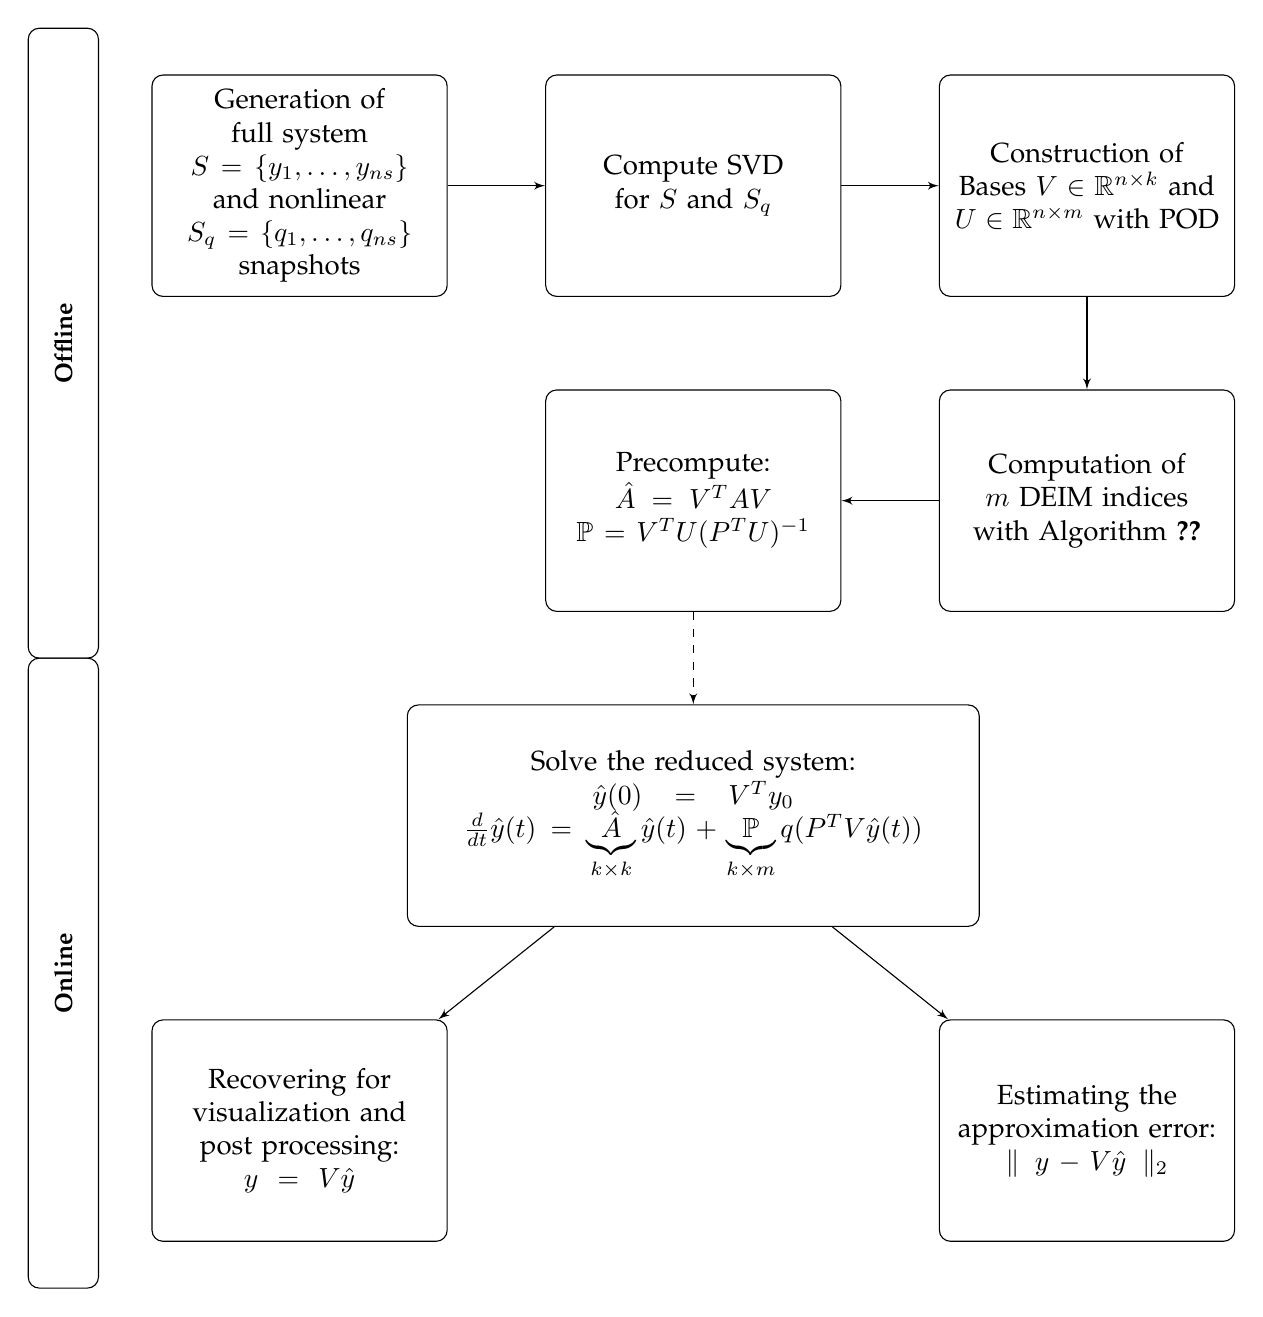
\begin{tikzpicture}[node distance = 3cm, auto]
    % Place nodes
    \node [block] (init) {Generation of full system $S=\{ y_1,\dots,y_{ns}\}$ and nonlinear $S_q =\{ q_1,\dots,q_{ns}\}$ snapshots};
    \node [block, right of=init ,node distance=5cm] (svd) {Compute SVD for $S$ and $S_q$};
    \node [block, right of=svd,node distance=5cm] (identify) {Construction of Bases $V \in \mathbb{R}^{n \times k}$ and $U \in \mathbb{R}^{n \times m}$ with POD};
    \node [block, below of=identify, node distance=4cm] (evaluate) {Computation of $m$ DEIM indices with Algorithm \ref{Chapter2:deim_algorithm}};
    \node [block, left of=evaluate, node distance=5cm] (update) {Precompute: \\$\hat{A} = V^TAV$\\  $\mathbb{P}=V^TU(P^TU)^{-1}$};
    \node [blocklong, below of=svd, node distance=8cm] (stop) {Solve the reduced system: \\$\hat{y}(0) = V^T y_0 $\\ $
  \frac{d}{dt}\hat{y}(t) = \underbrace{\hat{A}}_{k \times k}\hat{y}(t)+ \underbrace{\mathbb{P}}_{k \times m} q(P^TV\hat{y}(t))$};
     \node [block, below of=init, node distance=12cm] (recovering) {Recovering for visualization and post processing: \\ $y = V\hat{y}$ };
     \node [block, below of=identify, node distance=12cm] (error) {Estimating the approximation error:\\ $\parallel y - V\hat{y}\parallel_2$  };
    % the labels on the left
    \begin{scope}[xshift=-3cm,yshift=-2cm]
        \node[mylabel] (offline)  {\rotatebox{90}{Offline}};
        \node[mylabel, below of=offline, node distance=8cm] (online) {\rotatebox{90}{Online}};
    \end{scope}
    % Draw edges
    \path [line] (init) -- (svd);
    \path [line] (svd) -- (identify);
    \path [line] (identify) -- (evaluate);
    \path [line,dashed] (update) -- (stop) ;
    \path [line] (evaluate) -- (update);
    \path [line] (stop) -- (recovering);
    \path [line] (stop) -- (error);

\end{tikzpicture}
\end{center}
\caption{An overview on the workflow of model reduction.}
 \label{Chapter2:workflowdeim}
\end{figure}


\begin{table}[H]
\begin{center}


$\begin{array}{|c|c|}
\hline
\text{compute Snapshots} & \text{Problem dependent} \\
  \text{SVD for POD-basis} & \mathcal{O}(nn_s^2) \\
  \text{DEIM algorithm for m interpolation indices} & \mathcal{O}(m^4+nm) \\
  \text{Precompute: } \hat{A} = V^TAV & \mathcal{O}(NNZk+nk^2)  \text{ for a sparse A} \\
  \text{Precompute: } \mathbb{P} = V^TU(P^TU)^{-1} & \mathcal{O}(nkm + m^2n + km^2 + m^3)\\
\hline
\end{array}$
\end{center}
\caption{Computational Complexity of POD-DEIM}
 \label{Chapter2:tablecomplex}
\end{table}


 

\chapter{Application of the POD-DEIM approach to a marine ecosystem model} % Main chapter title

\label{Chapter3} % For referencing the chapter elsewhere, use \ref{Chapter1} 

%----------------------------------------------------------------------------------------

\section{Introduction}
To apply the POD-DEIM approach on a marine ecosystem model, the Simulation Package Metos3D (a Marine Ecosystem Toolkit for Optimization and
Simulation in 3-D) \cite{metos3dsimpack} is used. This package provides the possibility to simulate the ocean circulation coupled with biogeochemical processes. 
For the simulation of the ocean circulation the package uses transport matrices as described in \cite{Khatiwala2005}. 
The matrices are extracted from a general circulation model (GCM) and are capturing the complex three-dimensional
advective diffusive transport of tracers in a GCM as a sparse matrix. 
The so called transport matrix method (TMM), demonstrated in \cite{TMM}, makes use of these pre-computed transport data to apply it on arbitrary variables. 
Monthly averaged diffusion and advection matrices, which are interpolated during computation, are used as a compromise between storage and accuracy.
The effects, that are in longitudinal and latitudinal directions, are treated explicitly while the vertical effects are computed implicitly. 
Thus, there are twelve explicit and twelve implicit matrices.  

In addition to this linear part, the package provides an interface for different 
biogeochemical models that vary in the number of tracers and types of modeled processes.
They are controlled by a set of parameters $u$ and describe processes like nutrient consumption as well as growing, dying and sinking of different tracer elements.
For example, the N-Model, that is used in Chapter \ref{Chapter4}, calculates the uptake of inorganic nutrients by phytoplankton of an implicit pyhtoplankton concentration in the euphotic zone (cf. \cite{biomodels}). 
This uptake is limited by the amount available inorganic 
nutrients and by the light. The model uses phosphate ($PO_4$) as tracer element which governs the rate of growth of pyhtoplankton.  


The surface grid has a resolution of $2.8125 ^{\circ}$ in both directions, longitudinal and latitudinal. This results into a $128 \times 64$ 
grid with 4448 horizontal points in the oceans, if the grid points, where only land is, are left out. Each grid point represents a water column, called profile. Each profile has at most 15 vertical depth layers.
Overall, there are $ n_h = 52749 $ grid points, which are held in 
one single vector for each tracer. The implicit and explicit matrices are extremely sparse as they have only 672k (0,024\%) and 5407k (0,19\%) non zero values. To solve a system with more than one tracer, the matrices and tracers 
are arranged in a block diagonal system. Thus, with each tracer the linear system grows.

The temporal resolution is $\Delta t = 1/2880$. Assuming a year with 360 days, $\Delta t$ represent a step of three hours. The boundary data is used to have the ice cover and latitude information for each profile and a domain data set
provides the model with the information of the depths and heights of the vertical layers of each profile. 

The packed provides two solver for periodic steady-states one is a fixed point iteration (spin-up) and the other a Newton solver. In this thesis only the spin-up solver is used.


\section{Reduce the System}
As said, the full discrete representation of the iteration for n tracers is a block diagonal system. An iteration
reads
\begin{equation}\label{metos_equ}
y_{j+1} = A_{impj} (A_{expj} y_j + \Delta t q_j(y_j,u,b_j,d_j)),
\end{equation}
where $y_j = (y_i(t_j))^n_{i=1}$ is a vector combined of all n tracer vectors and $t_j = t_0 + (j-1)* \Delta t$ is a point in time.
$A_{impj}$ and $ A_{expj}$ are the
block diagonal matrices, interpolated for the time index $j$. The discrete boundary and domain data is represented by
$b_j = (b_i(t_j))^{n_b}_{i=1}$ and $d_j = (d_i(t_j))^{n_d}_{i=1}$. The biogeochemical model $q_j$ is described by
$q_j(y_j,u,b_j,d_j) = (q_i(t_j,y_i,u,b_i,d_i))^n_{i=1}$.

To apply the POD-DEIM approach, let $n=1$, so that there is only one tracer and let $n_h$ be the length of the tracer vector. The basis matrices $V \in \mathbb{R}^{n_h \times k}$
and $U \in \mathbb{R}^{n_h \times m}$ are computed with the POD method. The projector $\mathbb{P} = U(P^TU)^{-1}P^T$ is computed
with the result $P \in \mathbb{R}^{n_h \times m}$ of the DEIM-Algorithm with input $U$.

After projecting the system \eqref{metos_equ} onto $V$ and applying the DEIM approximation onto the nonlinear part, it
reads
\begin{equation}\label{metos_equ_projected}
 \hat{y}_{j+1} = V^TA_{impj} (A_{expj}V \hat{y}_j + \Delta t    \mathbb{P} q_j(V \hat{y}_j,u,b_j,d_j)),
\end{equation}
where $\hat{y}_j = V^T y_j$.

To use the advantage of the reduction, $V^TA_{impj}$ is multiplied out and the system looks like this:
\begin{equation}\label{metos_red}
\begin{aligned}
 \hat{y}_{j+1} &= \underbrace{V^TA_{impj} A_{expj}V}_{A_{rj} \in \mathbb{R}^{k \times k}} 
 \hat{y}_j + \Delta t  \underbrace{V^TA_{impj} U(P^TU)^{-1}}_{\mathbb{P}_rj \in \mathbb{R}^{k \times m}} P^T q_j(V \hat{y}_j,u,b_j,d_j)
  \\ &= A_{rj} \hat{y}_j + \Delta t    \mathbb{P}_{rj} P^T q_j(V \hat{y}_j,u,b_j,d_j).
 \end{aligned}
\end{equation}
 
The matrices $A_{rj}$ and $\mathbb{P}_{rj}$ are interpolated out of the twelve monthly average matrices $A_{ri}$ and $\mathbb{P}_{ri}$ for $i = 1,...,12$.
$A_{ri}$ and $\mathbb{P}_{ri}$ are precomputed out of monthly averaged matrices $A_{impi}$ and $A_{expi}$ of the original system,
the POD-basis $V$ as well as $U$ and the DEIM index matrix $P$. Thus, $A_{ri} = V^T A_{impi} A_{expi} V$ and
$\mathbb{P}_{ri} = V^T A_{impi} U(P^TU)^{-1}$. They are dense, but quite small, because $k<<n_h$ and $m<<n_h$.

\subsection{Reduction of the nonlinear part}
The reduction of the nonlinear part is more complex. The best reduction would be possible if the nonlinear function could be evaluated componentwise. Then, only 
the selected points have to be computed and the reduction would be from $n_h$ to $m$ evaluations.
But in Metos3D the biogeochemical model is evaluated independently for each profile.


Thus, to compute one point a whole profile has to be evaluated. The profiles that have to be evaluated can be calculated with 
the help of the DEIM-indices and the land-sea mask which contains the geometry information.
From all the $p=4448$ profiles of the full-order model (FOM), only $m$ are computed. Thus, the dimension reduction is less
than the reduction of the linear part but one evaluation of the biogeochemical model can be very expensive.  
 
The following pseudo code describes the reduced evaluation of the nonlinear function.
\begin{algorithm}
\caption{Pseudo code for the reduction of a biogeochemical model}\label{Chapter3:deim_algorithm}
\begin{algorithmic}[1]
   \item \textbf{Input: }{$\vec{\varrho} = \{\varrho_1,..,\varrho_m\}^T \in \mathbb{N}^m$}
   \item \textbf{Output: }{$\hat{q} \in \mathbb{R}^m$} 
   \For{$i=0 $ to $m$}
      \State $index = \textbf{range of profile in tracer vector for DEIM-point } \varrho[i]$ 
      \State $y_p = V[index,:] \hat{y}$ 
      \State $b_p,d_p$ = \textbf{select corresponding boundary and domain conditions}
      \State $q_p = q(y_p,u,b_p,d_p)$
      \State $\hat{q}[i] = q_p[\varrho [i]]$ 
    \EndFor
\end{algorithmic}
\end{algorithm}

This algorithm uses the DEIM-indices as input and provides an evaluation of the biogeochemical model at the desired points.
In line 4 the range of the profile for a specific DEIM-point is determined, and then, this part of the high dimensional tracer
is computed, through projection with the POD-basis $V$. After selecting the corresponding boundary and domain conditions
the biogeochemical model function is evaluated for this profile. In line 8, the desired point in the profile is
saved and the rest of the vector is discarded. 


Overall, for one time step of the reduced model, the steps that are described by Algorithm \ref{Chapter3:reduced_algorithm} have to be done.
\begin{algorithm}
\caption{pseudo code for time step of reduced model}\label{Chapter3:reduced_algorithm}
\begin{algorithmic}[1]
  \item \textbf{Input: } {$\textbf{point in time } t \in [0,1)$, $\hat{y}_j \in \mathbb{R}^k$}
 \item \textbf{Output: } {$\hat{y}_{j+1} \in \mathbb{R}^k $}
 \State \textbf{compute $\hat{q}$ with Algorithm \ref{Chapter3:deim_algorithm}}
 \State $\textbf{ interpolate } A_{ri} \textbf{ and } \mathbb{P}_{ri} \textbf{ in point } t$
 \State $\hat{y}_{j+1} = A_{ri}\hat{y}_j + \mathbb{P}_{ri} \hat{q}$ 
\end{algorithmic}
\end{algorithm}

For one time step, the desired parts of the biogeochemical model have to be evaluated, and then, two matrix
vector multiplications have to be done. 


\section{Implementation}
The code to generate the reduced-order models was mainly written in python using scipy and numpy \cite{scipy}. The DEIM Algorithm and the precomputing of the system matrices were implemented
with numpy. To exchange data with the PETSc library, used by Metos3D, IO routines for PETSc files were created in python. 

To compute the SVD of the snapshot matrices, at first, numpy was used. 
As the matrices have become quite large during the progress of this thesis, and the SVD algorithm in numpy was not suitable
for matrices of this size, the library SLEPc \cite{slepc-toms} was used.
This provides the possibility to compute partial SVDs in parallel. The algorithms SLEPc uses are explained in \cite{svd_parallel}, where a performance analysis is given as well. 

The reduced model was implemented in python. The biogeochemical models used in Metos3D were included directly with F2PY (Fortran to Python interface generator).

The whole code is freely accessibly via
\begin{equation*}
 \text{\url{https://github.com/neeljp/MasterThesis_POD-DEIM}}
\end{equation*}
and can be used for further improvements or demonstration.











 















\chapter{Numerical Examples} % Main chapter title}
\label{Chapter4} 
In this chapter the results of numerical experiments with different biogeochemical models are presented. First an investigation of the one tracer N-Model will be presented. 
Starting with an overview about how many snapshots have to be taken into account to build an accurate reduced-order model (ROM). Afterwards, information about the accuracy and CPU time of ROMs from the N-Model with different POD-DEIM base dimension
are given. In Chapter \ref{behaviorofroms} different ROMs of the N-Model are compared to the full-order model (FOM) in terms of convergence, relative error and speed up. 
Building up on these results the behavior of ROMs for the N-DOP-Model is investigated and compared to the full-order N-DOP-Model, in Chapter \ref{numerical_n-dop}.


%----------------------------------------------------------------------------------------

\section{Experiments with N-Model}
\label{Chapter4_N} 
\begin{figure}[!ht]
\centering
  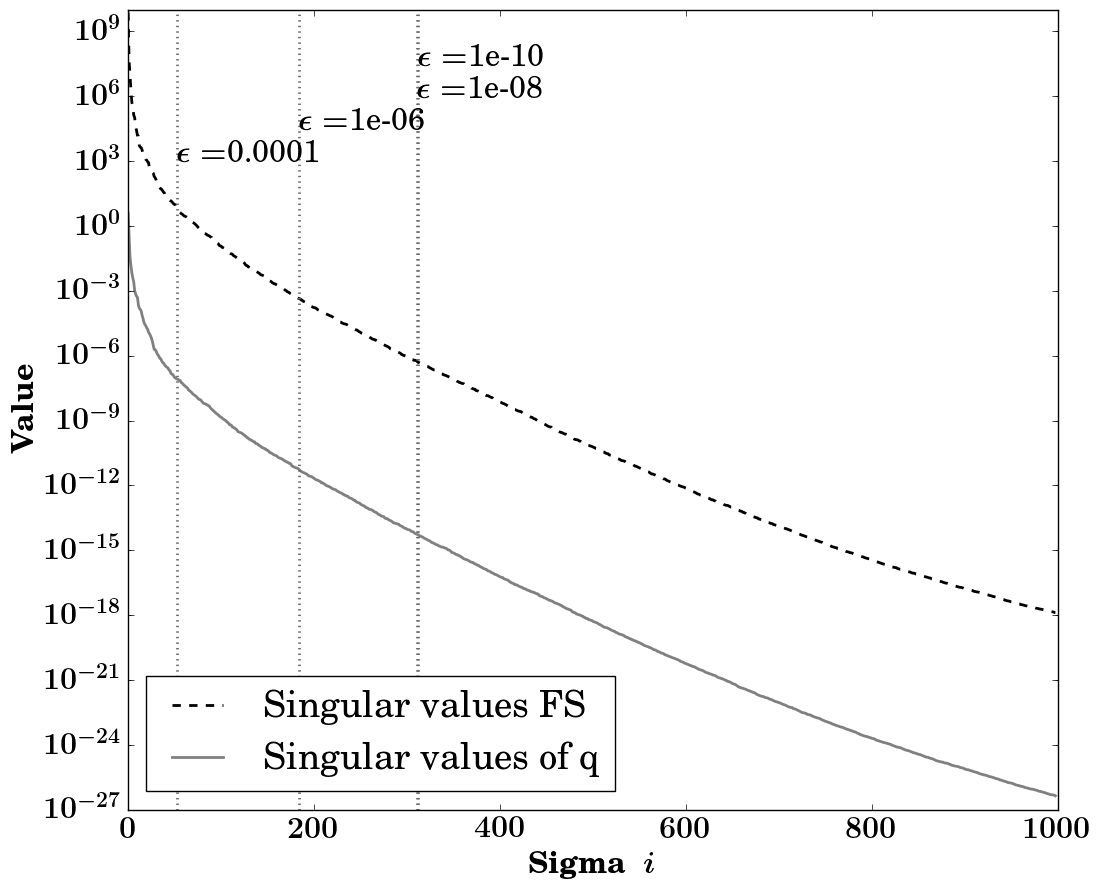
\includegraphics[width=0.6\textwidth]{singularvalues_full_trajectory.png}
  \caption{Distribution of singular values from a SVD of $12\_3000$, a matrix of snapshots distributed over the whole year.}
  \label{fig:singularvalues_full_trajectory}
\end{figure}

The first experiments were done with a one tracer model, the so called N-model
in Metos3D. To test and show the feasibility of the reduction a specific fixed parameter set $u_r =\{0.02,2.0,0.5,30.0,0.858\}$ was used to generate snapshots. These
parameters are taken from \cite{metos3dsimpack}, where they are given as the parameter set of a reference solution. A  uniformly distributed start concentration of $2.17\frac{mmol}{m^3}$ was used.
The time scale was set to $6000$ model years and three model states in each month were saved. The reason to only save three states out of the 2880 in one year, was the size of the data. One state vector used $0.422KB$ and two have to be save for each state, one for the full system and the other one for the nonlinear part. Thus, storing 2880 snapshots would have taken
$2.37GB$ per year.
Therefor, it was tried to reduced the amount of snapshots taken.
Different snapshot matrices were build from these saved states to try out how many must be taken to build an accurate reduced-order model (ROM). 

Figure \ref{fig:singularvalues_full_trajectory} shows the distribution of the first 1000 singular values from an SVD of a snapshot matrix  $S = \{y^{i}_1,\ldots,y^{i}_{3000}\}$ for $i =1,\ldots,12$ (called $12\_3000$). These snapshots are distributed uniformly over
the whole year and are taken at the end of each month, thus $12 \times 3000 = 36000$ snapshots were taken. 
The solid line are the singular values of the nonlinear snapshots and the dashed line are the ones from the snapshots of the full system. 
These two behave very similar, independently from the choice of the snapshot distribution.
The vertical dotted lines point out the estimated dimension $k$ of the base with a POD error $\epsilon$, computed with \eqref{Chapter2:eq:error_funcion_pod}.
It shows that an $\epsilon < 10e-8$ does not change $k$ anymore. 

\begin{figure}[H]
\centering
  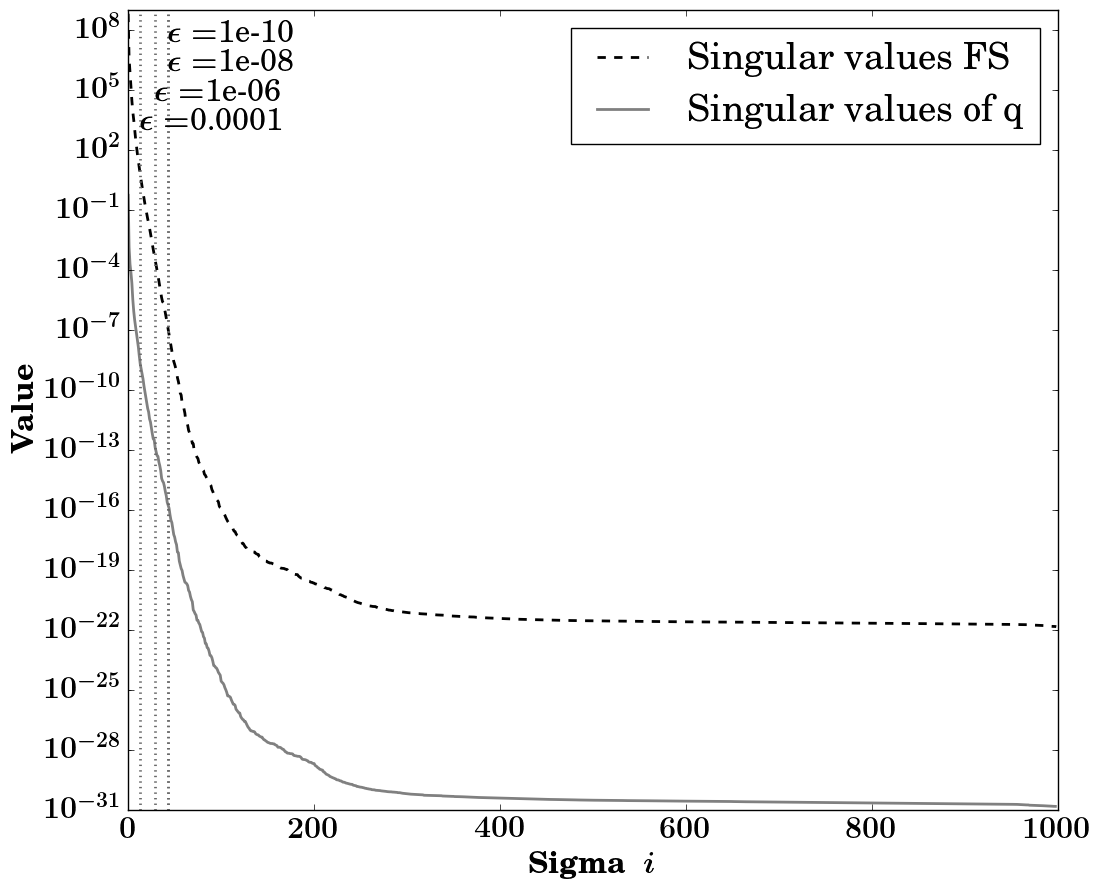
\includegraphics[width=0.6\textwidth]{singularvalues_one_month.png}
  \caption{Distribution of singular values from an SVD of $3\_3000$ a matrix of snapshots taken only in winter.}
  \label{fig:singularvalues_one_month}
\end{figure}

In comparison with Figure \ref{fig:singularvalues_one_month} the singular values descend slowly. There the singular values of an SVD from $S = \{y^{1}_1,y^{2}_1,y^{12}_1,\ldots,y^{1}_{3000},y^{2}_{3000},y^{12}_{3000} \}$  (called $3\_3000$)
are plotted. In the literature \cite[][p. 261]{ROM_Book} it is written that fast decaying singular values are a requirement for constructing efficient ROMs and
are an indicator for the quality of the ROM.


The snapshots for the singular values in Figure \ref{fig:singularvalues_one_month} were taken only in winter. The distribution seems to be more feasible for a ROM, but since
only data in winter time were taken into account, the ROM resulting from the corresponding singular vectors is inaccurate in summer time, as shown in Figure \ref{fig:error_one_month}. 
It shows that at least one snapshot in each month has to be used because otherwise the reduced model will leak accuracy in the months that are left out. There the relative error
\begin{equation}\label{eq:relativeError}
 \mathcal{E} = \parallel y^{FO}_j - y^{RO}_j \parallel_2/ \parallel y^{FO}_j \parallel_2
\end{equation}
over the period of a whole year from two different bases is plotted. The one, where only snapshots in winter
time contributed to the base, (dashed line) has an increasing error in summer time, which leads to a drifting of the solution. The other one (dotted line), where the snapshots were distributed over the whole year, is more accurate and has nearly the same error over the course of the entire year.

\begin{figure}[H]
\centering
  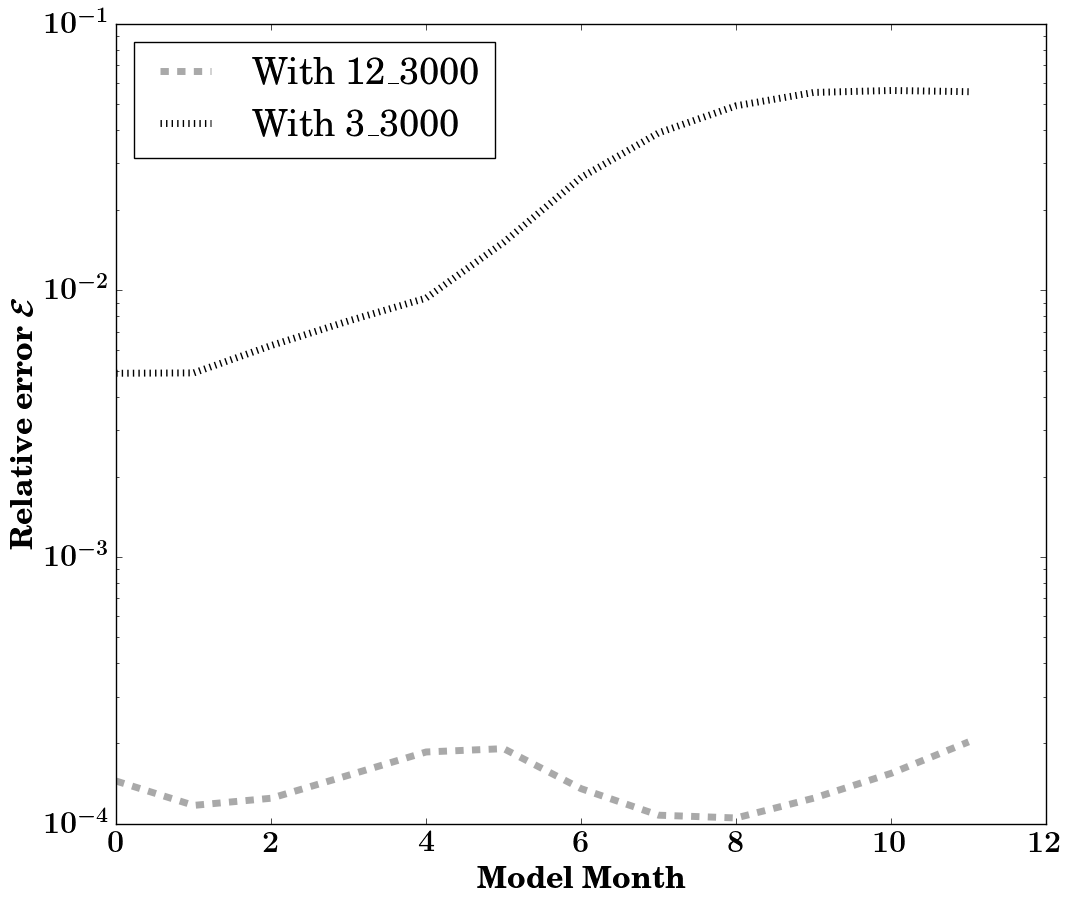
\includegraphics[width=0.6\textwidth]{relative_error_one_month.png}
  \caption[Relative error $\mathcal{E}$ during the course of a year for two different bases.]{Relative error $\mathcal{E}$ during the course of a year for two different bases. One where the Snapshots where taken in winter only and the other with snapshots distributed over the whole year.}
  \label{fig:error_one_month}
\end{figure}
Comparing the plots of the different singular values in Figure \ref{fig:comparison_differnt_singuarvalues} with the relative error of the
derived ROMs in Figure \ref{fig:relative_error}, it is not possible to see the correlation of the quality of the ROM with the singular values as proposed in the literature.
Interesting is that the singular values of $12\_3000$ and $12\_6000$ are very similar and the behavior of the derived ROMs is similar as well, 
as shown in Figure \ref{fig:spinup} and \ref{fig:relative_error}. This indicates that taking snapshots after 3000 model years into the snapshot set does not change the ROM.
Thus, it is sufficient to take only snapshots from the first 3000 model years, but it is better to take more snapshots during the course of the model years.

\begin{figure}[H]
\centering
\begin{subfigure}{.5\textwidth}
  \centering
  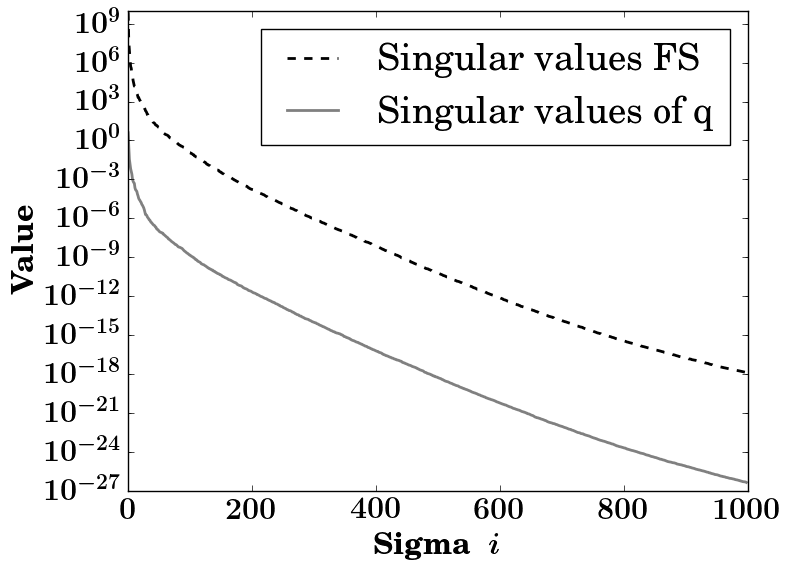
\includegraphics[width=1\textwidth]{singularvalues_12_3000.png}
  \caption{$12\_3000$}
  \label{fig:sing_sub1}
\end{subfigure}%
\begin{subfigure}{.5\textwidth}
  \centering
  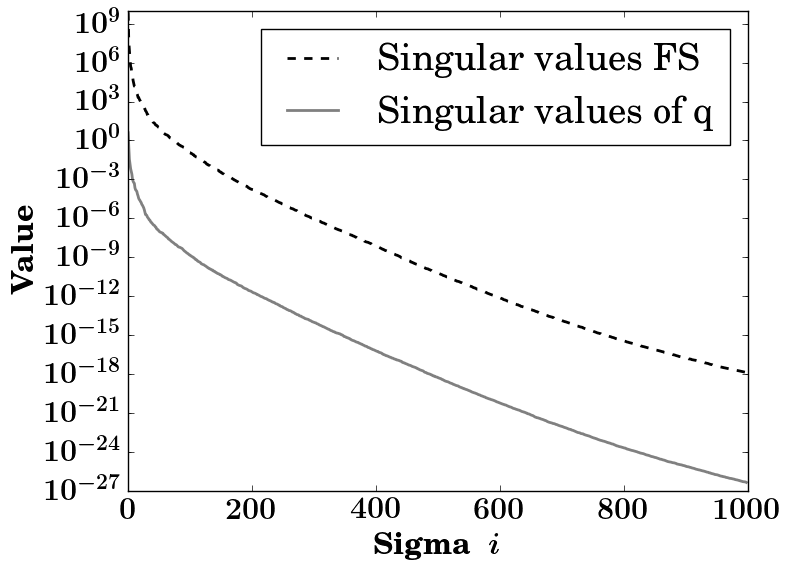
\includegraphics[width=1\textwidth]{singularvalues_12_6000.png}
  \caption{$12\_6000$}
  \label{fig:sing_sub2}
\end{subfigure}
\begin{subfigure}{.5\textwidth}
  \centering
  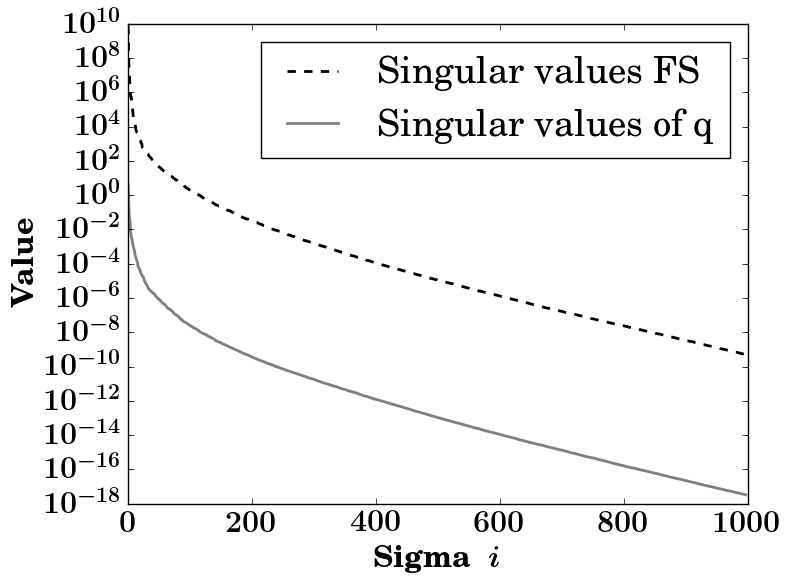
\includegraphics[width=1\textwidth]{singularvalues_36_1000.png}
  \caption{$36\_1000$}
  \label{fig:sing_sub3}
\end{subfigure}%
\begin{subfigure}{.5\textwidth}
  \centering
  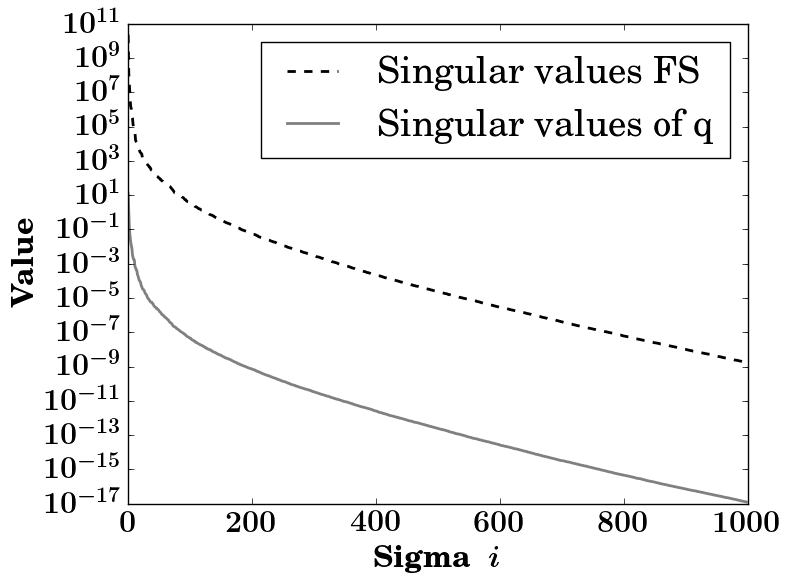
\includegraphics[width=1\textwidth]{singularvalues_36_3000.png}
  \caption{$36\_3000$}
  \label{fig:sing_sub4}
\end{subfigure}
\caption{Distribution of singular values from an SVD of different snapshot matrices.}
\label{fig:comparison_differnt_singuarvalues}
\end{figure}






\subsection{Approximation error and CPU time}\label{approxerrocputime}
To find out how to choose the dimension of the POD and the DEIM basis, a row of experiments were made. The singular vectors for these bases come from the SVD of uniformly distributed snapshots over 3000 model years ($12\_3000$), see Figure \ref{fig:singularvalues_full_trajectory}
for the corresponding singular values. In these experiments the size of one base was fixed and the size of the other one was changed. The size of a base marks the number of left singular vectors of the SVD that are taken to build the base. 
In Figure \ref{fig:comparison_differnt_pod_diem}
the behavior of the average relative error 
\begin{equation}\label{arerror}
\bar{\mathcal{E}} = \frac{1}{n_t} \sum\limits_{j=0}^{n_t}{ \parallel y^{FO}_j - y^{RO}_j \parallel_2/ \parallel y^{FO}_j \parallel_2}
\end{equation}
with $n_t = 1000$ is shown on the left. Either the DEIM dimension is fixed (black with dots) at $m=150$ or the POD dimension $k=150$ is fixed (gray with diamonds). It can be seen that both lines are limited to
the same accuracy and also the error of a ROM with both bases dimension of $300$ (gray star) does not lead to a better
approximation. The fixed POD ROMs reach that point as the dimension of the DEIM base is larger than $40$. Below that the approximation
gets worse. The fixed DEIM ROMs converge slower at a POD base size of $130$. Thus, chose the size of the POD base around $
130$ and the DEIM base around $40$ could be sufficient for the accuracy of the ROM. Note that, in this case, only information from the first 1000 model years are used and for longer model runs this might change.

\begin{figure}[H]
\centering
\begin{subfigure}{.5\textwidth}
  \centering
  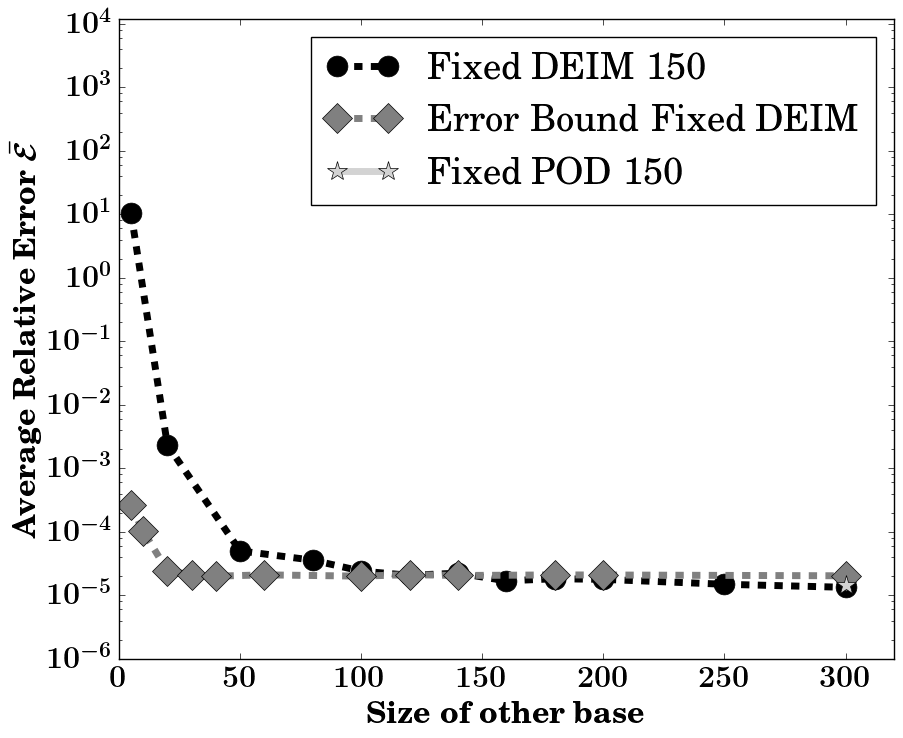
\includegraphics[width=1\textwidth]{realative_error.png}
  \caption{Relative error}
  \label{fig:compare_sub1}
\end{subfigure}%
\begin{subfigure}{.5\textwidth}
  \centering
  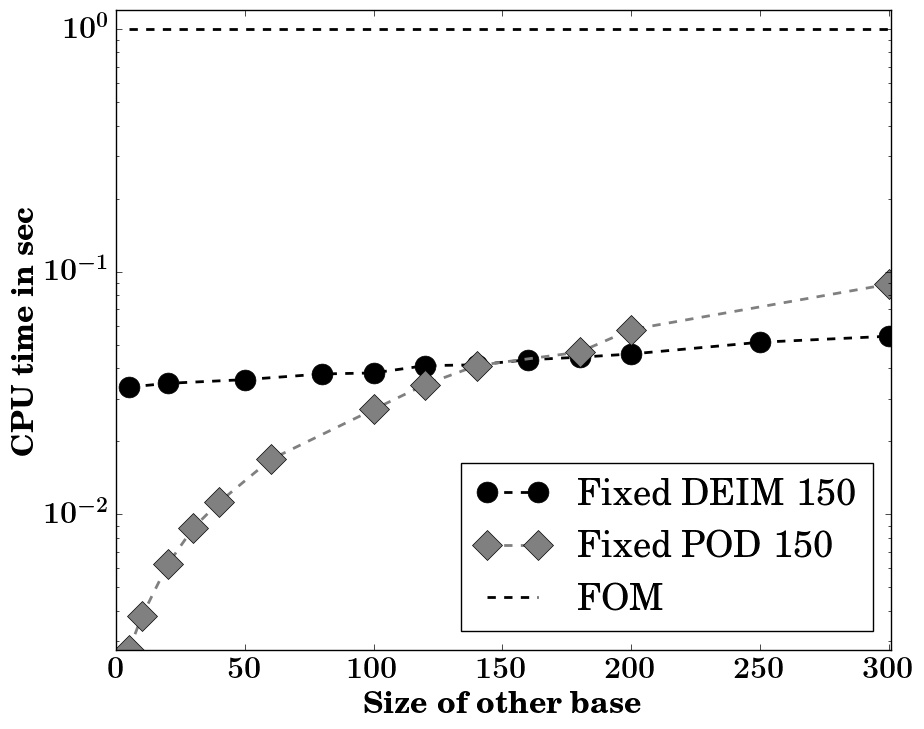
\includegraphics[width=1\textwidth]{avarage_cpu_time.png}
  \caption{Average scaled CPU time}
  \label{fig:compare_sub2}
\end{subfigure}
\caption[The average relative error and the average CPU time of different ROMs of the N-Model.]{The average relative error \eqref{arerror} of different ROMs is shown on the left side and average CPU time for these ROMs on the right.}
\label{fig:comparison_differnt_pod_diem}
\end{figure}


On the right side of Figure \ref{fig:comparison_differnt_pod_diem} the average CPU time for one model year of these ROMs with different base sizes is shown. The CPU time was taken over 1000 model years and scaled with the time of the 
full-order model (FOM). The black line with dots, where the size of the POD base changes, indicates that a large POD base does not lead to 
a strong increment of CPU time for the whole system. whereas changing the size of the DEIM base leads to a noticeable change in CPU time, as shown by the gray line with diamonds. This was made with
a one tracer model and will change with more tracers since the amount of matrix vector multiplications in \eqref{metos_red} will grow linear with the number of tracers. 
Overall a speed up between $10$ and $100$ is possible. For the minimal size of the bases, derived from the left side in Figure \ref{fig:comparison_differnt_pod_diem},
the speed up would be close to $100$. 
In Figure \ref{fig:error_bound} the real average relative error of the bases is compared to the approximated error bound of the POD-DEIM approach from Chapter \ref{Chapter2}.
The bounds are quite pessimistic, but they show a similar behavior as the real error, if the base size changes. There it is even better to see that the error of the POD part is
governing the error of the whole system. 
\begin{figure}[H]
\centering
  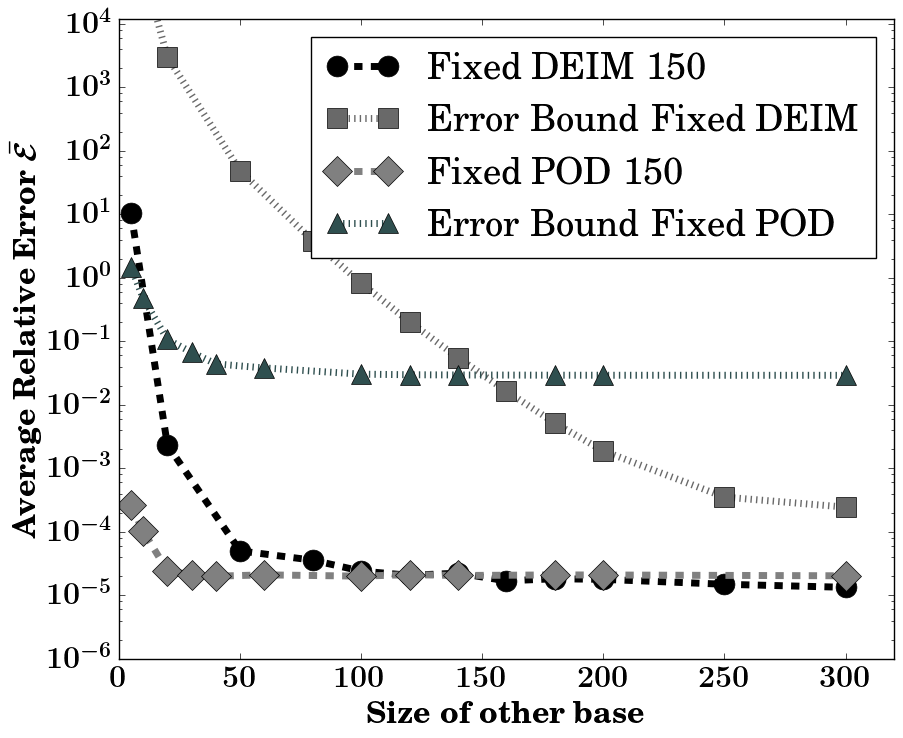
\includegraphics[width=0.7\textwidth]{realative_error_bound.png}
  \caption{The average relative error $\bar{\mathcal{E}}$ compared to the error bounds \eqref{ch2:error_bound_pod},\eqref{ch2:error_bound_deim} of the POD-DEIM approach.}
  \label{fig:error_bound}
\end{figure}
In conclusion, increasing the DEIM base size over the size of the POD base does not lead to a better approximation, but this increases the CPU time a lot. The increase of size of the POD base over the size of the DEIM instead does lead to a
decreasing approximation error. Therefore, the size of the POD base should be chosen larger than the size of the DEIM base or 
at least they should have the same size.

\subsection{Behavior of the Reduced-Order Models}\label{behaviorofroms}

In order to explore the convergence and the error behavior of different bases long simulations were made. 
The base names begin with the name of the SVD, i.e. $12\_3000$, which means 12 snapshots per year and 3000 years of data. Then follows a pattern like $P100D50$, where $P100$ means a POD basis of dimension $k=100$ and $D50$ means a DEIM basis of dimension  $m=50$.
At first, the convergence towards a periodic steady state was tested and compared to the convergence behavior of the full-order model.
In Figure \ref{fig:spinup} the spin-up norm 
\begin{equation}\label{eq:spinupnorm}
 S_{norm} = \parallel y_l - y_{l-1} \parallel_2 
\end{equation}
is plotted, which is the norm of the difference between the initial states of consecutive model years $l$.
It shows that none of the ROMs reaches a periodic steady state.
The full-order model reaches a periodic steady state after about 7000 model years, as shown in Figure 2 in \cite{metos3dsimpack}.


\begin{figure}[H]
\centering
  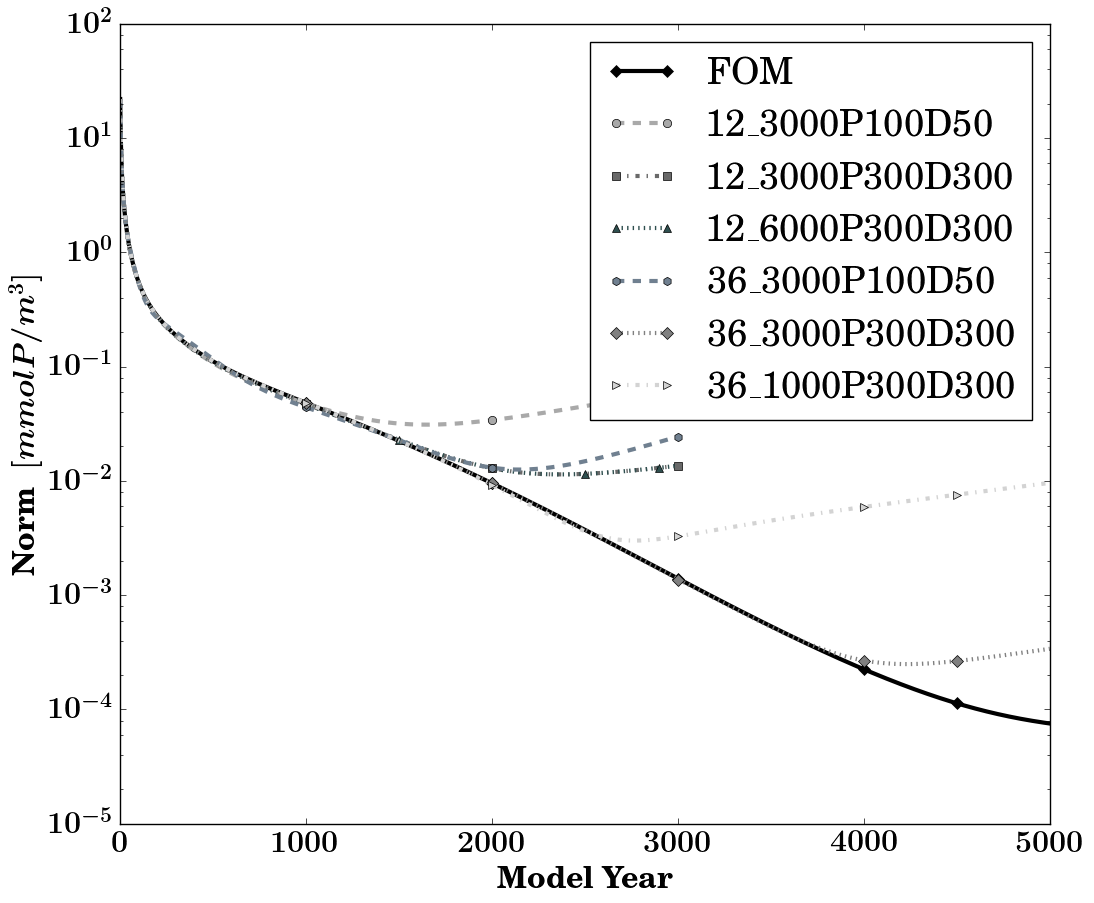
\includegraphics[width=0.8\textwidth]{spinupnorm_base_compare_2.png}
  \caption{Spin-up norm of different reduced-order models in comparison with the spin-up norm of the full-order model.}
  \label{fig:spinup}
\end{figure}
All ROMs diverge at some point. The ROM out of $12\_3000P100D50$ starts to deviate first, at about 1000 model years, form the black line, which
shows the spin-up behavior of the full-order model. The ROMs $12\_3000P300D300, 12\_6000P300D300$ and $36\_3000P100D50$ depart after 1500 model years and
begin to diverge. The ROM $36\_3000P100D50$ increases faster than the other two because of the smaller size of the bases. The ROM derived 
from the longer timeline of snapshots behaves in the same way as the base that is derived from only snapshots out of 3000 model years.
The ROM $36\_3000P300D300$ is the last one that departs from the behavior of the FOM, after about 3800 model years. This is far away from the other ones which show similar behavior.  
The ROM derived from only snapshots of 1000 model years diverges at around 2500 model years, this is later than the $12\_3000P300D300$ ROM. This indicates again that taking more snapshots during the year is more important than the total number of years 
that are taken into account.


Figure \ref{fig:relative_error} shows the relative error \eqref{eq:relativeError} of the same bases. The error was measured over 3000 model years and was computed the end of each year.
All ROMs show an increasing error over the 3000 years. Again the ROMs $12\_3000P300D300$ and $12\_6000P300D300$ show a similar behavior and the ROM out of $12\_3000P100D50$ has the largest error and the fastest increase.


\begin{figure}[H]
\centering
  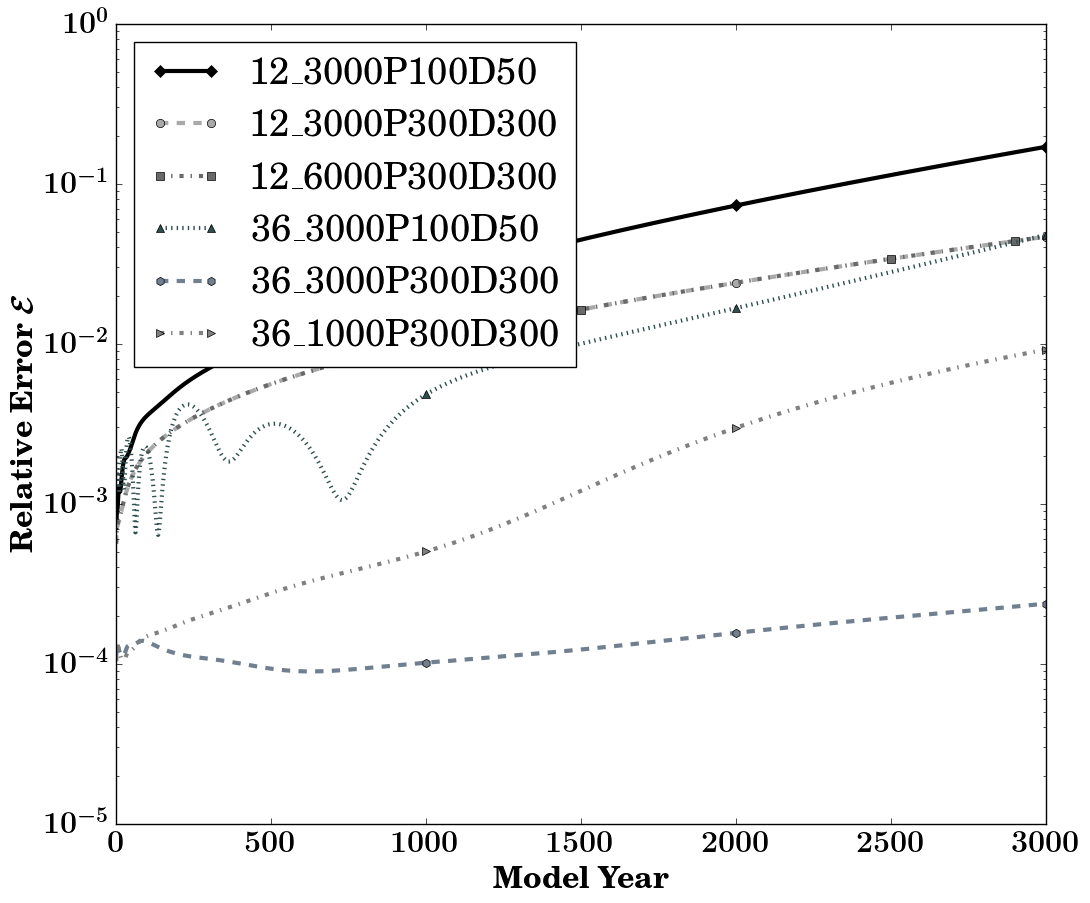
\includegraphics[width=0.8\textwidth]{error_norm_base_compare_2.png}
  \caption{Relative error $\mathcal{E}$ of different reduced-order models.}
  \label{fig:relative_error}
\end{figure}

The error of all ROMs oscillates at the beginning, usually only the first 100 model years, but the error of $36\_3000P100D50$ has a strong oscillation until 1000 model years.
Afterwards, it shows the same increase as the black line of $12\_3000P100D50$. The ROM $36\_3000P300D300$ shows the slowest error increment as well as a
very different behavior in the first 500 model years. At first, it oscillates as well, but only a couple of model years, after that it slightly decreases until around 600 model years.
Then the increment starts, but it is much slower than that of the other ROMs. The base $36\_1000P300D300$, where only snapshots from the first 1000 model years were taken, starts 
with the same error as $36\_3000P300D300$, but shows a stronger increment over the model years.

In conclusion, large bases have a better convergence behavior and a smaller approximation error. Taking snapshots throughout a longer time period than 3000 model years does not change the convergence behavior nor the relative error. Indeed, changing the amount of snapshots per year influences both.


To show some more quantities of the ROMs, four bases have been picked out and compared in Table \ref{Chapter4:table}.
The bases are generated out of two different snapshot sets, one is the set $36\_3000$, the other is the set $36\_1000$.
For each of them two bases are selected with different POD and DEIM base sizes.
For each of them the following quantities have been measured:
\begin{itemize}
 \item $t_{setup}$ - The time which is required to pre-compute the SVD, the DEIM indices and the matrices $A_{ri}$ and $P_{ri}$. Note that this only has to be performed once. 
 The SVD was computed with SLEPc on an Intel\textsuperscript{\textregistered} Sandy Bridge EP architecture with Intel Xeon\textsuperscript{\textregistered}  E5-4640 that consist of 8 cores running at 2.4 GHz. The DEIM indices and the base matrices with 
 Intel Core\textsuperscript{\textregistered} i7-4750HQ that consist of 8 cores running at 2 GHz. They where computed sequentially and the SVD was computed with 96 cores in parallel.
 \item $S_P$ - The speed up for a model year, which is the ratio of the computational time for a model year of the FOM and the ROM. They were both computed sequentially on the i7-4750HQ.
 \item $M_{a}$ - The relative mass change of the model after $a$ years, scaled with the total mass of the tracer at $t=0$, i.e. $\frac{\parallel V_{y_a} \parallel_1 - \parallel V_{y_0} \parallel_1}{\parallel V_{y_0} \parallel_1}$, where $V_{y_a}$ is a vector 
 of the masses of the tracer $y_a$. 
 \item $\bar{\mathcal{E}}_{a}$ - The average relative error \eqref{arerror} over $a$ years. 
 \item $\bar{\mathcal{E}}_{*}$ - The approximated error bound of the POD-DEIM approach as defined in Chapter \ref{Chapter2}. 
 \item $R_{a}$ - The number of spin-ups (model years) that the FOM needs to get to the solution of 3000 model years, if initialized with the output of the ROM at model year $a$. 
\end{itemize}

\begin{table}[H]
\begin{center} 


$\begin{array}{|l|c|c|c|c|c|}
\hline
\text{SVD} & \multicolumn{2}{c|}{36\_3000} & \multicolumn{2}{c|}{36\_1000} & - \\
\hline
\text{Base}  & P100D50 & P300D300  & P100D50 & P300D300  & FOM\\
\hline t_{setup} [s]  & (9676,10,39) & (9676,870,327) & (2071,9,38) & (2071,989,350) & -\\

\hline S_P  & 78.29 & 7.35  & 73.00 & 9.08 & -\\

\hline M_{1000}  & 0.00227 & 0.00019  & 0.00102 & 0.00056 & 0.00013\\

\hline M_{3000}  & 0.03727 & 0.00056  & 0.25539 & 0.00725 & 0.00039\\

\hline \bar{\mathcal{E}}_{1000}  & 0.00252 & 0.00010  & 0.00156 & 0.00029 & -\\

\hline \bar{\mathcal{E}}_{3000}  & 0.01409 & 0.00014  & 0.06661 & 0.00250 & -\\

\hline \bar{\mathcal{E}}_{*}  & 77.35 & 0.11475  & 44.72 & 0.05972 & -\\

\hline R_{1000}  & 2028 & 1995  & 2114 & 1996 & -\\

\hline R_{3000}  & 1711 & 40  & 2755 & 758 & -\\
\hline
\end{array}$
\end{center}
\caption{Comparison of four ROMs from the N-Model}
 \label{Chapter4:table}
\end{table}
The time to set up the ROMs is dominated by the computation of the SVD, which is only possible because only a truncated SVD was computed in parallel.
In the 9676 seconds (2.6h)  and 2071 seconds (0.57h) two SVDs were computed, one for the POD method and one for DEIM. The time
to compute the DEIM indices grows fast with the size of the DEIM base because of the complexity of the Algorithm \ref{Chapter2:deim_algorithm}.

The relative mass change for the $P100D50$ ROMs is much higher than that of the $P300D300$. 
It is increasing from 1000 to 3000 model years for all of the ROMs.
The $36\_3000P300D300$ has nearly the same mass change as the FOM. 
The average relative error is increasing a lot from 1000 to 3000 model years, except for the $36\_3000P300D300$ ROM. The approximated error bound $\bar{\mathcal{E}}_{*}$ is not accurate and roughly three orders of magnitude away from the 
real error. It indicates that the $36\_1000$ ROMs should be more accurate than the $36\_3000$ ROMs. This is due to the fact that the smaller snapshot matrix has smaller singular values and the approximated error bound relies mostly 
on the singular values.

If the output solution of one of the ROMs after 1000 model years were taken and the FOM is initialized with them, the FOM needs nearly the rest of the 3000 model years to
get to the original solution. If the output of the ROMs after 3000 model years is taken only the ROM $36\_3000P300D300$ supplies a solution that is
near the one after 3000 model years of the FOM. The other are far away, even further away as the solution at 1000 model years as for the
ROM $36\_1000P100D50$, which takes 2755 model years in the FOM. If it is done like this, i.e. combining one ROM with the FOM, all the systems will give an overall speed up of approximated 1.4, if supplied with the ROM solution of 1000 model years.
The system supplied with the solution after 3000 model years of the ROM $36\_3000P300D300$ will only need time equivalent to $\frac{3000}{7.35}  + 40 = 447$ model years of the FOM to get to the original solution of 3000 model years.
This leads to an overall speed up of $\frac{3000}{447} \approx 6.71$.
Note that here CPU times of different implementations are compared, the FOM is implemented in C with PETSc and the ROM is implemented in python with numpy and both were run sequentially.
It is expected to get a better speed up if the ROM will be implemented in C as well.

In conclusion, the creation of a reduced-order model of the N-Model is feasible and the POD-DEIM leads to an adequate reduction in
computational cost. As long as the snapshots and reduced matrices only have to be computed once and then the reduced system is solved
many times with them. This leads to the question whether it is possible using one reduced model for different sets of parameters and get accurate solutions.
This problem will be described in Chapter \ref{Chapter5}. In the next chapter the reduction of a two tracer model is explained and
the results of experiments with it are presented.




\section{Experiments with N-DOP-Model}\label{numerical_n-dop}
The model used in these experiments uses two tracer elements. It extends the N-model, which considers only inorganic phosphate ($PO_4$ called $N$ here) with dissolved
organic phosphorus (called DOP). All uptake of phosphate is shifted either to export production or to DOP in this model. It is further described in
\cite{biomodels}. The model uses one vector for each tracer, and thus, there are two solution vectors.
36 uniformly distributed snapshots per year from the first 1000 model years were generated. For this the parameter set $u= \{0.02,2.0,0.5,30.0,0.67,0.5,0.858\}$  was used and the start concentration was set to $2.17\frac{mmol}{m^3}$ and $1e^{-4} \frac{mmol}{m^3}$, for N and DOP respectively.
There are two strategies how to create a ROM for this model, one is to create one snapshot matrix out of the combined tracers vectors, i.e. 
\begin{equation*}
S = \left [
\begin{array}{ccc}
\vertbar &        & \vertbar \\
 y^N_1 &  \ldots & y^N_{ns}\\
 \vertbar &        & \vertbar \\
  \vertbar &        & \vertbar \\
 y^{DOP}_1 & \ldots& y^{DOP}_{ns}\\
 \vertbar &         & \vertbar \\
\end{array} \right ].
\end{equation*}
The other option would be to create two independent matrices 
\begin{equation*}
S_N = \left [
\begin{array}{ccc}
 y^N_1 &  \ldots & y^N_{ns}\\
\end{array} \right ], \quad
 S_{DOP} = \left [
\begin{array}{ccc}

 y^{DOP}_1 & \ldots& y^{DOP}_{ns}\\

\end{array} \right ]
\end{equation*}
and create one POD-DEIM base for each tracer. 
The first one has not lead to a usable ROM because the DOP solution vector was tremendously inaccurate. A possible reason might be the fact that the DEIM algorithm has picked out indices only in the upper part of the combined vector, thus, in the $y^N$ part.
Consequently, for the nonlinear part only information from the solution of one tracer were taken into account. Thus, the part of other tracer were only bad approximated.

In the following, the results of the second, decoupled approach are presented. Therefore, a matrix with 36 equally distributed snapshots for each model year over 1000 model years was created and the 
SVD was computed. The singular values of both tracers in Figure \ref{fig:singularvalues_N-DOP} look similar to those from the N-Model. Thus, it is expected that the resulting ROM will give similar results as well.

\begin{figure}[H]
\begin{subfigure}{.48\textwidth}
  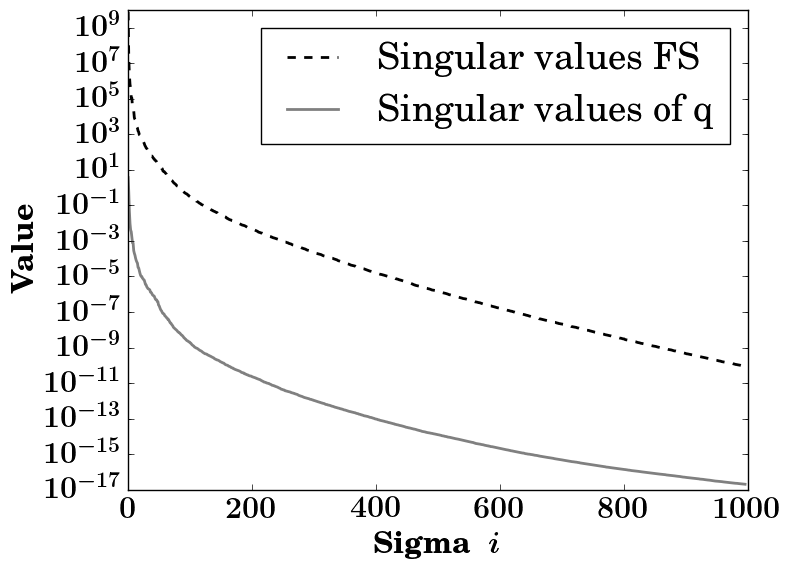
\includegraphics[width=1\textwidth]{singularvalues_N-DOP_1000_N.png}
  \caption{Singular values of $S_N$}
  \label{fig:sing_N-DOP_sub1}
\end{subfigure}%
\begin{subfigure}{.5\textwidth}
  \centering
  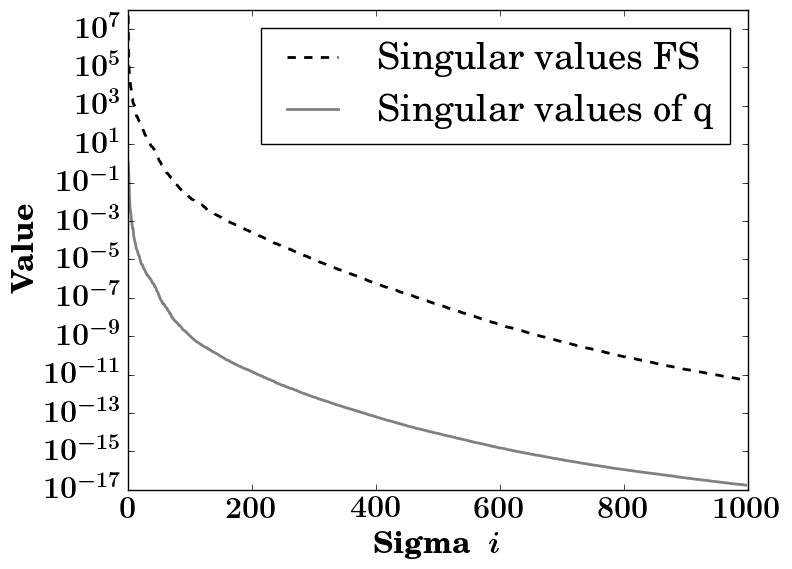
\includegraphics[width=1\textwidth]{singularvalues_N-DOP_1000_DOP.png}
  \caption{Singular values of $S_{DOP}$}
  \label{fig:sing_N-DOP_sub2}
\end{subfigure}
\caption{Distribution of the singular values of 36\_1000 from the N-DOP-Model.}
\label{fig:singularvalues_N-DOP}
\end{figure}

In Figure \ref{fig:spinup_N-DOP} the spin-up norm \eqref{eq:spinupnorm} of two ROMs of the N-DOP-Model is shown for each tracers. 
The ROM with the smaller base matrices shows a very different spin-up behavior than the FOM. Both tracer concentrations
are oscillating during the first 500 model years. 
\begin{figure}[ht]
\centering
  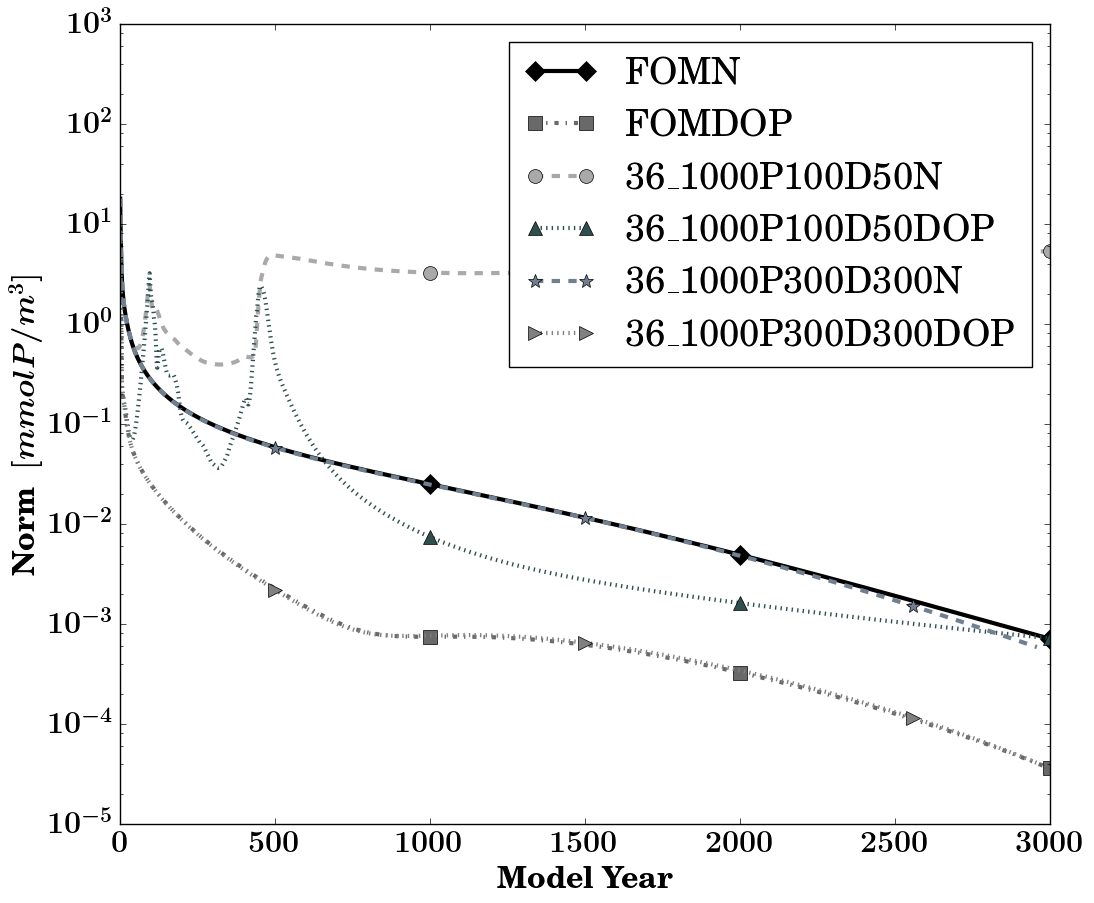
\includegraphics[width=0.8\textwidth]{spinupnorm_base_compare_N-DOP.png}
  \caption{Spin-up norm of two ROMs in comparison with the spin-up norm of the FOM of N-DOP.}
  \label{fig:spinup_N-DOP}
\end{figure}
Afterwards, the N concentration is changing a lot from model year to model year, but the change
does not increase. The DOP concentration converges to a state with only small changes each model year.
The other ROM, that is shown in Figure \ref{fig:spinup_N-DOP}, has nearly the same change of concentration over the 3000 model years as the FOM. This is interesting because
the ROM was only created with information of the first 1000 model years and such a ROM of the N-Model diverges stronger from the FOM, compare Figure \ref{fig:spinup}.

The relative error \eqref{eq:relativeError} over 3000 model years for each tracer of these ROMs is presented in Figure \ref{fig:relative_error_N-DOP}.
First of all, note that in this case it relates to a relative error and values higher than one mean that the error is larger than the 
2-norm of the original solution vector of the FOM. Thus, the error of both concentrations (N,DOP) of the smaller ROM is large compared to 
the overall concentration in the FOM, and the N part shows a strong increasing over the model years. The DOP part is nearly constant after one peak at about 500 model years.
Since the relative error of the ROM $36\_1000P100D50$ increases far beyond one after 500 model years, 
the solution of this ROM is not close to the solution of the FOM.
\begin{figure}[ht]
\centering
  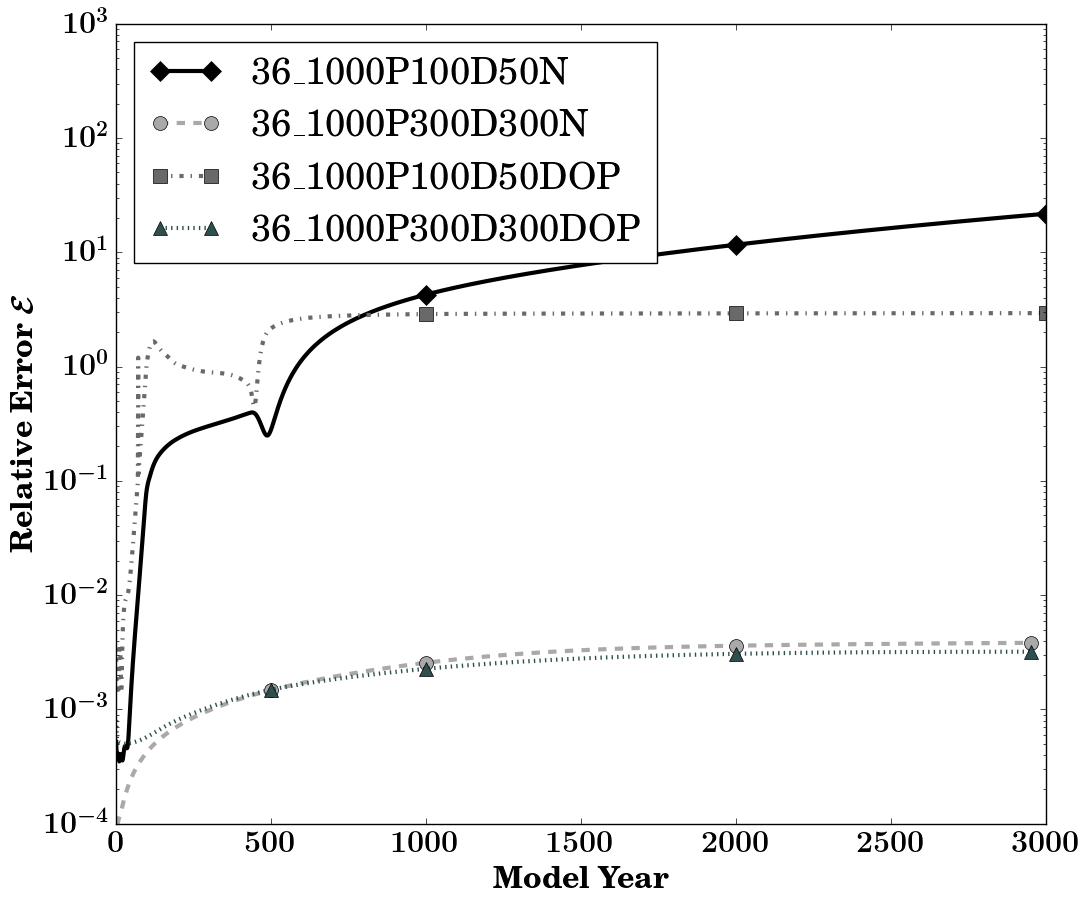
\includegraphics[width=0.8\textwidth]{error_norm_N-DOP.png}
  \caption{Relative error $\mathcal{E}$ of two ROMs of the N-DOP-Model.}
  \label{fig:relative_error_N-DOP}
\end{figure}
The relative errors of both concentrations of the 
ROM $36\_1000P300D300$ are increasing over the 3000 model years, at first, stronger and later they stay nearly constant. 
The are both very similar in each model year and in an order of $10^{-3}$.

Table \ref{Chapter4:table-N-DOP}
shows the same information as Table \ref{Chapter4:table} for the N-DOP-Model. The setup times of the 
ROMs are roughly doubled because each tracer has its own bases, and thus, its own setup process. Due to this fact the speed up is much smaller as well.
Since each tracer has its own and mostly different DEIM indices, the biogeochemical model has to be evaluated 
nearly twice the number of DEIM indices. In the ROM $36\_1000P300D300$ only 52 DEIM indices of the two tracers were identical, this is less then 10\%.
In addition, the number of matrices that must be interpolated is doubled as well because each tracer has its own
POD base. For a comparison of the CPU time of the main operations during one time step of the N-Model and the 
N-DOP-Model look in Appendix \ref{Appendix:cpupie}.

The relative mass change in the DOP concentration is tremendously high in all models as well as in the FOM, but the mass change of the ROM $36\_1000P300D300$ is nearly equal to that of the FOM. 
Note that the start concentration of DOP is $1e^{-4} \frac{mmol}{m^3}$, and thus, it has a really low amount of substance compared to the start concentration of N.
The N part of the model $36\_1000P300D300$ has less mass change than the FOM. This mass change becomes
even smaller after 3000 model years than after 1000, although, the mass change usually increases over the course of the model years.

The relative error of the ROM $36\_1000P100D50$ is higher than one as well after 1000 as after 3000 model years and for both tracers.
Supplying the solution of this ROM into the FOM, it does not come near the the original solution of 3000 model years within the
time of 3000 model years. Basically this results because of the poor approximation of the ROM, the resulting high relative mass change of the system, as well as the occurrence of
a lot negative concentration values. For DOP$\approx 75 \%$ and for N$\approx 1\%$ compared to approximately  $47\%$ and $0\%$ negative values in the solution of the
FOM after 3000 model years. The approximated error bounds for the ROMs are much closer to the actual error than in the N-Model.
The approximated error bound for the DOP tracer is lower than the actual error in both ROMs.
Since the tracers interact with each other, it is a question that has to be answered, whether the error bound of each tracer gives information about the error of the whole system.

The error of the ROM $36\_1000P300D300$ is similar in both tracers, and it is comparable to the error of the 
same sized ROM of the N-Model. The solution of this model is usable to produce a solution with the FOM that is close to the original solution. 
The FOM takes 2011 and 495 spin-ups to get to the original solution and with this setup a speed up of 1.7 is possible. This is less than the speed up of the
N-Model which depends mostly on the fact that a separate POD-DEIM base is used for each tracer.  
Overall, the POD-DEIM approach can be applied to the N-DOP-Model and the other multi tracer models, if a separate POD-DEIM base is used for each tracer.

\begin{table}[H]
\begin{center} 


 $\begin{array}{|l|c|c|c|c|c|c|}
 \hline
 
\text{Base}  & \multicolumn{2}{c|}{36\_1000P100D50} & \multicolumn{2}{c|}{36\_1000P300D300} & \multicolumn{2}{c|}{FOM}\\
\hline t_{setup} [s]  & \multicolumn{2}{c|}{3965,19,69} &\multicolumn{2}{c|}{3965,1989,646} & \multicolumn{2}{c|}{-}\\
\hline S_P  & \multicolumn{2}{c|}{14.47323} & \multicolumn{2}{c|}{2.42209}  & \multicolumn{2}{c|}{-} \\
\hline

\text{Tracer}  & N & DOP & N & DOP & N & DOP\\

\hline M_{1000}  & 2.607 & 1039.21  & 0.00652 & 184.282 & 0.00854 & 183.912\\

\hline M_{3000}  & 18.192 & 1073.76  & 0.00550 & 186.397 & 0.00874 & 185.631\\

\hline \bar{\mathcal{E}}_{1000}  & 1.293 & 1.803  & 0.00143 & 0.00142 & - & -\\

\hline \bar{\mathcal{E}}_{3000}  & 8.325 & 2.543  & 0.00279 & 0.00243 & - & -\\


\hline \bar{\mathcal{E}}_{*}  & 6.517 & 0.38633  & 0.00862 & 0.00044 & - & -\\

\hline R_{1000} &  \multicolumn{2}{c|}{-} &  \multicolumn{2}{c|}{2011} &  \multicolumn{2}{c|}{-} \\
\hline R_{3000} &  \multicolumn{2}{c|}{-} &  \multicolumn{2}{c|}{495} &  \multicolumn{2}{c|}{-} \\
\hline
\end{array}$


\end{center}
\caption{Comparison of two ROMs from the N-DOP-Model}
 \label{Chapter4:table-N-DOP}
\end{table}
In the next chapter the results of experiments with ROMs of the N-Model for parameter studies are presented.

%\section{Experiments with MITgcm-PO4-DOP-Model}
%\label{Chapter4:mitgcm}




 
% Chapter Template

\chapter{Experiments for Parameterized Reduced Order Models} 
\label{Chapter5}

The previous examples showed the feasibility to use the POD-DEIM approach on marine ecosystem models with a fixed 
set of parameters. In \cite{PODDeimapplication}, the authors propose to use the POD-DEIM approach for parameter studies of dynamical 
systems. In this case, it means to simulate the full-order model for multiple parameter sets and
use all the snapshots to create a reduced-order model. To investigate this the N-Model with one tracer is used again, but this time with different parameter sets. Since the parameter space is quite large, 
Latin Hypercube sampling, as proposed in \cite{ROM_book2}, is used to generate ten samples (cf. Table \ref{Chapter5:table_lhc_sample}) within the bounds
that are given in Table 2 in \cite{metos3dsimpack}. In Chapter \ref{Chapter4}, the amount of snapshots for the smallest setup of viable ROM was $36 \cdot 1000= 36000$ snapshots.
Thus, for every parameter sample 36000 snapshots are used. Since a SVD must be computed of the whole 
snapshot matrix, there exist a soft upper bound for the number of snapshots, and thus, for the number of parameter samples.
The combined snapshot matrices are
\begin{equation*}
 S =[Y_1|\dots|Y_9], \quad S_q = [Q_1|\dots|Q_9],
\end{equation*}
where $Y_i$ and $Q_i$ are the snapshot matrices of the solution corresponding to the Latin Hypercube sample $i$.
These are in total 360000 snapshots, thus, the matrices $S$ and $S_q$ have the dimension $52749 \times 360000$.
The singular values of this SVD are visible in Figure \ref{fig:singularvalues_10_lhc}. They decrease much slower than the ones in Figure \ref{fig:comparison_differnt_singuarvalues} from the N-Model.
\begin{figure}[ht]
\centering
  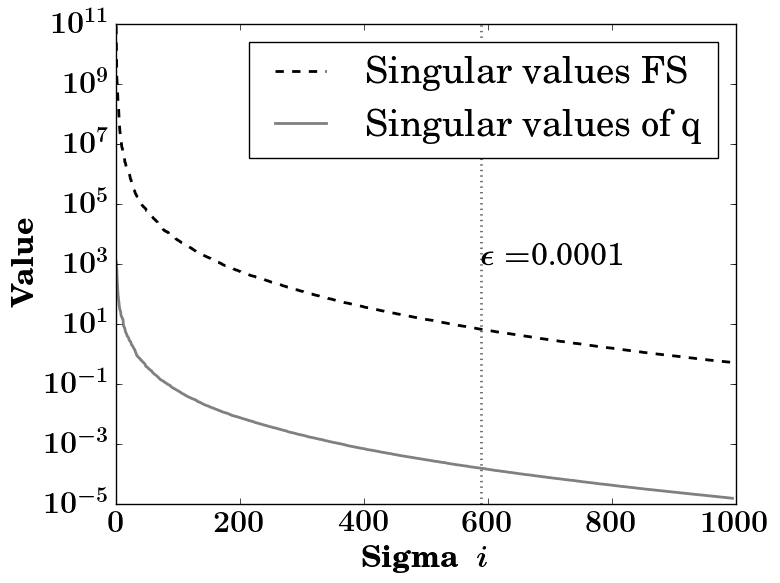
\includegraphics[width=0.7\textwidth]{singularvalues_10_lhc_1000.png}
  \caption{Distribution of singular values of $S$ and $S_q$.}
  \label{fig:singularvalues_10_lhc}
\end{figure}
The singular values of the full system matrix decent only to a value near $10^0$, this is much higher than the previously showed singular values.
The approximated error bound of a ROM, created out of the corresponding left singular vectors, is tremendously high, in an order of $10^4$.
It was not possible to create a ROM that generates a solution that is close to the original for any of the parameter sets listed in Table \ref{Chapter5:table_lhc_sample}, with which the model was created. The relative 
error is always over 1 and it is oscillating a lot in the course of 3000 model years, cf. Figure \ref{fig:error_norm_lhc_0}. With a new parameter set that was not used to create the model, for example 
$1.5 \cdot u_r = u_r + 50\% = \{0.03,3.,0.75,45.,1.287\}$, the result is similar. The ROM, created out of multiple solution trajectories, is very inaccurate, cf. Figure \ref{fig:error_norm_+50}.
Thus, the approach to create one ROM out of multiple trajectories seems not to lead to an accurate and useful one. One possible explanation for this is the diversity of the solutions that the FOM generates for different parameter sets.
Together, they can not be well approximated within the same low dimensional subspace. Therefore, the subspace, generated by the POD method, is only a poor approximation. 

Another idea is to create multiple ROMs for multiple parameter sets. And then for a new parameter set use the ROM that was created with the parameter set that is the closest to the new one. 
This approach should be possible if a ROM can produce an acceptable solution also for a set of parameters 
that is different from the parameter set the ROM has been created with.
To try this out, four parameter sets are taken. The parameter sets are deviations from the reference parameter set $u_r + x\%$ with $x\in \{5,10,20,50\}$.
Using the ROM $36\_3000P300D300$, from Chapter \ref{Chapter4_N}, which was create with the parameter set $u_r$, simulation are made. 
The relative error between these spin-ups and the corresponding original solution of the FOM is shown in Figure \ref{fig:error_norm_one_base_+50}. In the figure it is visible that the further away the parameter set from $u_r$ is, the larger becomes the relative error of the solution of the ROM to the original solution of the FOM. 
All spin-ups show a decrease of the error in the first half of the 1500 model years and an increase in the second half of the 3000 model years. The further away the parameter set is, the earlier the relative error begins to increase. 
The relative error is in the order of $10^{-1}$, thus, the solution that the ROM generates for a different set of parameters, seems to be not usable.  
The dashed lines with the left arrow show the relative error between the two FOM spin-ups. One spin-up was executed with parameter set $u_r$ and the other spin-up was run with one of the deviations $u_r + x\%$. Plotted in order 5, 10, 20, 50 from bottom to top. Compared to corresponding relative error of the FOM, the solutions of the ROMs are most of the time less accurate. And it seems that carrying out a ROM simulation with a different set of parameters does not lead to a significant change in the solution. The change is larger, the further away the set of parameters is, but then, there is a stronger divergence after around 1000 model years.

\begin{figure}[ht]
\centering
  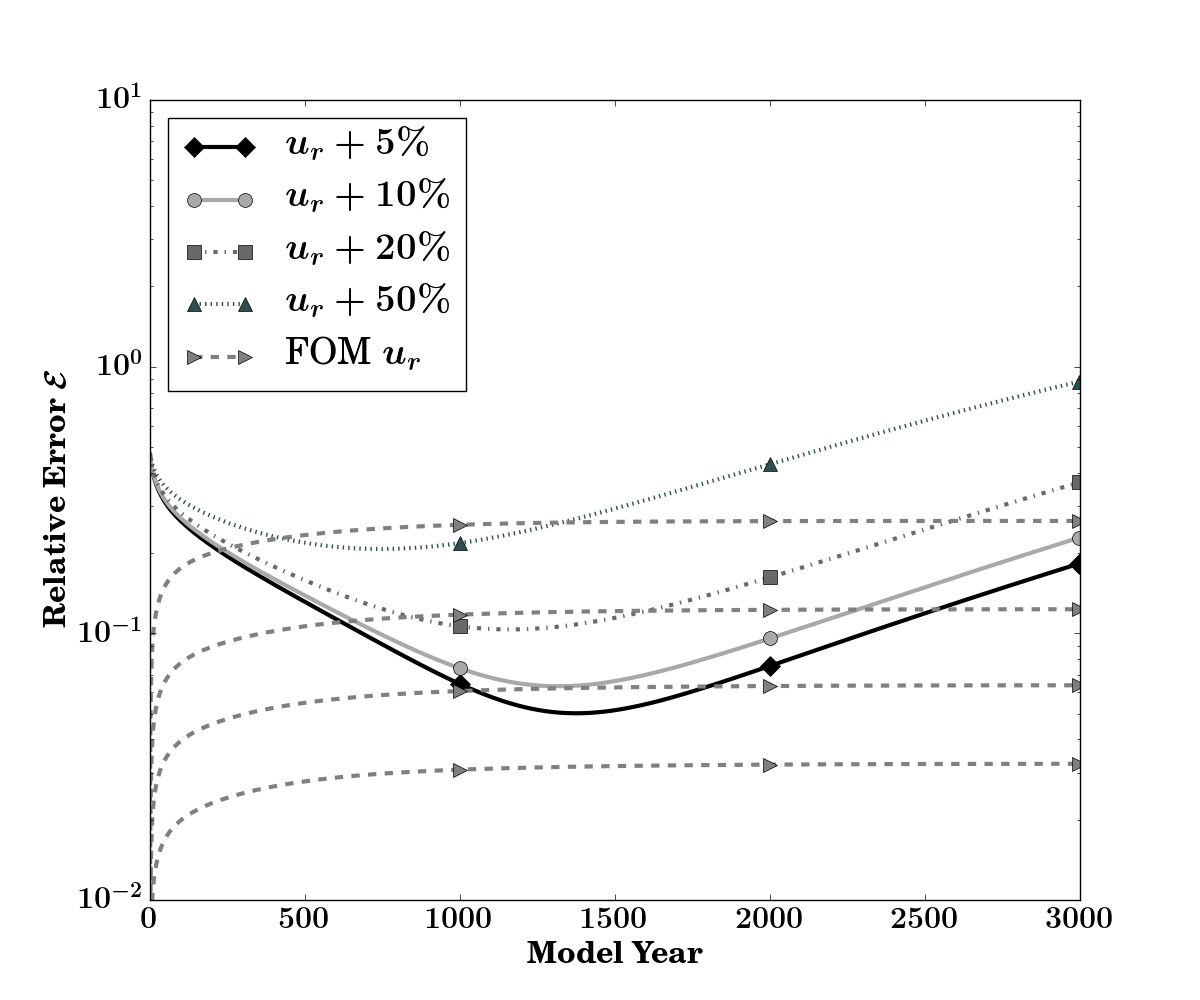
\includegraphics[width=0.9\textwidth]{error_norm_one_base_+50.png}
  \caption[The relative error between the ROM $36\_3000P300D300$ and the FOM for different sets of parameters.]{The relative error between the ROM $36\_3000P300D300$ and the FOM for different parameter sets $u_r + x\%$, where $x\in \{5, 10, 20, 50\}$. The dashed lines with the left arrow show the relative error between 
  the FOM spin-up with parameter set $u_r$ and one of the deviations $u_r + x\%$. Plotted in order 5,10,20,50 from bottom to top.}
  \label{fig:error_norm_one_base_+50}
\end{figure}

In Figure \ref{fig:error_norm_one_base_+50_FOM_+0}, the relative error between the ROMs spin-ups for the parameter sets $u_r + x\%$ with $x \in  \{5,10,20,50\}$ and the FOM solution of $u_r$ is visible. The error is
large, which means that the spin-ups of the ROM are not close to the original solution of the FOM using the parameter set $u_r$. Thus, the ROM results in a completely different solution if it is executed with a different parameter sample than it was created with and they start to diverge early. 

In conclusion, executing a ROM with a different set of parameter than it was created with does not lead to a usable solution. Thus, the idea of creating multiple ROMs and using them for parameter studies seems not to be feasible. Overall, it has not been possible to find a ROM or multiple ROMs that can be used for new sets of parameters and resulting in an acceptable solution.
\begin{figure}[ht]
\centering
  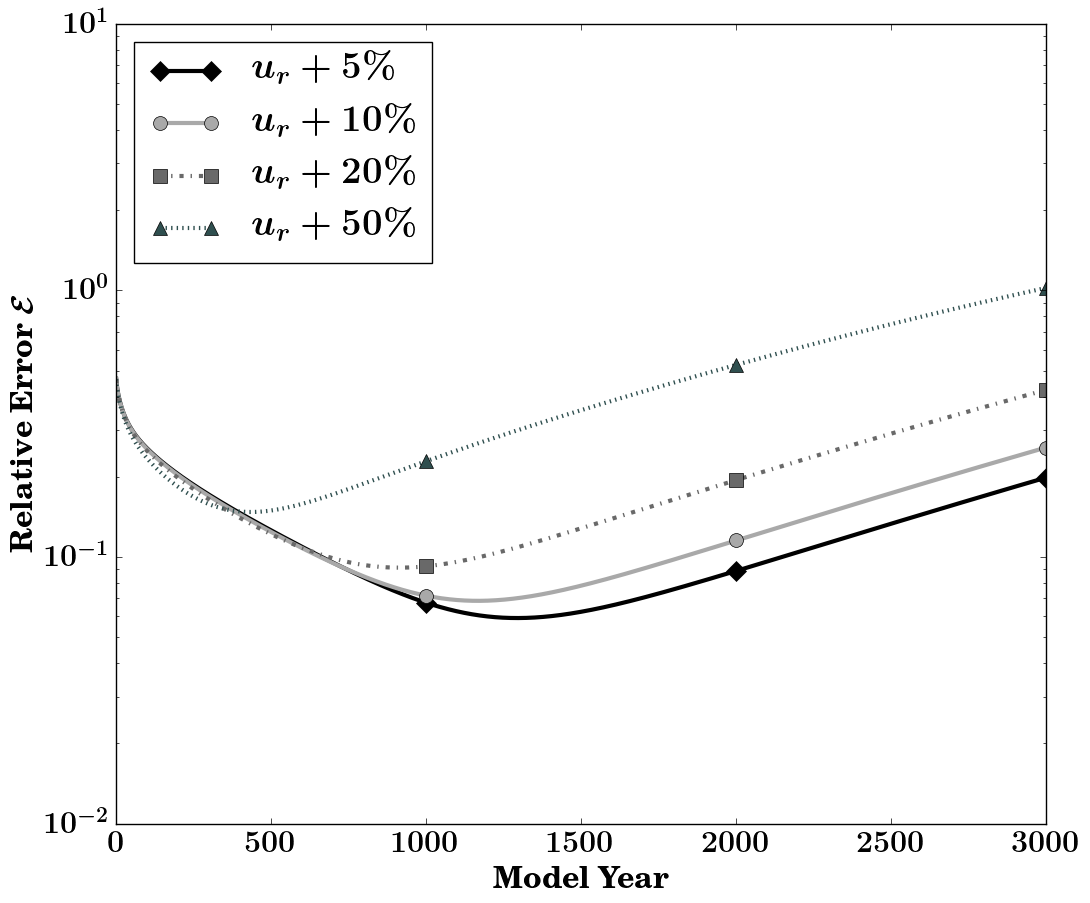
\includegraphics[width=0.9\textwidth]{error_norm_one_base_+50_FOM_+0.png}
  \caption[The relative error between the ROM $36\_3000P300D300$ and the FOM solution of $u_r$.]{The relative error between the ROM $36\_3000P300D300$ for the parameter sets $u_r + x\%$  and the FOM solution of $u_r$, where $x\in \{5,10,20,50\}$.}
  \label{fig:error_norm_one_base_+50_FOM_+0}
\end{figure}
 

\chapter{Conclusion and Future Work} % Main chapter title

\label{Chapter6} % For referencing the chapter elsewhere, use \ref{Chapter1} 

%----------------------------------------------------------------------------------------

\section{Conclusion}
In this thesis, the nonlinear MOR method POD-DEIM has been applied to three different marine ecosystem models of the software package Metos3D.
Therefore, the reduced model equations \eqref{metos_red} were established and implemented. Then, an analysis of the one
tracer model, the N-Model, was made, in which the feasibility was tested. 
For that the manner of how many information from the full-order model are needed for an accurate reduced-order model was investigated.
Moreover, it was examined how the size of the reduced bases affect the accuracy and CPU time of the reduced-order model.
On the basis of these results six reduced-order models of the N-Model were compared to the full-order model.
The approach was extended on the two tracer model, the N-DOP-Model, and two reduced-order models were compared to the full-order N-DOP-Model.
Afterwards, it was tried to create reduced-order models of the N-Model, which could be used for parameter studies.
For that two approaches were tested. The first one was to create a reduced-order model out of multiple trajectories created with different parameter sets.
And the other one was to use one reduced-order model for multiple parameter sets.


One main goal of this thesis was to demonstrate the feasibility of the nonlinear MOR method POD-DEIM on 
marine ecosystem models with respect to accuracy and computational speed up. The numerical experiments in Chapter \ref{Chapter4}
have demonstrated the feasibility for a fixed set of parameters. The POD-DEIM approach leads to a significant speed up and a solution that is close to that of the full-order model measured in the 2-norm. For the two tracer N-DOP-Model the speed up is smaller because of
the fact that a base for each tracer has to be used to get an accurate reduced-order model.


The idea of using the POD-DEIM approach to get a reduced-order model for parameter studies has turned out to be not practical.
The main reason for that is diversity of the solutions for different sets of parameters, and thus, 
the approximation within a low dimensional subspace is very inaccurate.


\section{Future Work}
At this point, some directions for future research, that might build
up on the work of this thesis, are presented. 

\subsubsection*{Selection of snapshots}


In Chapter \ref{Chapter4_N} the selection of snapshots for the SVD is not optimal and could be further improved.
Since there is no theoretical approach to optimize the selection, it is only possible with numerical experiments.
A problem in that area is the soft upper bound of the total number of snapshots that is given by the SVD algorithm.
For that the Algorithm 5.1 in \cite{PODDeimapplication} may be interesting.
This algorithm uses the Gram-Schmidt QR factorization with a reorthogonalization algorithm from \cite{Daniel2007ReorthogonalizationAS}.
The algorithm detects and eliminates redundant snapshots as well as prevents the loss of orthogonality of the POD basis due to the numerical instability of the Gram–Schmidt process.


\subsubsection*{Creating a reduced-order model for parameter studies}
For parameter studies it could be tried to create a reduced-order model only for a subset of the parameters, thus, changing only some parameters and leave the others fixed.
This could lead to a usable model since the space spanned by the solution should be smaller. Another idea is to create a reduced-order model for a subspace of the parameter space, thus, use all parameters but only create a model for 
parameters in the range of $u_r \pm x\%$. The idea is the same, the reduction of the solution space, and thus, a better low dimensional approximation. 

\subsubsection*{Create combined ROMs}
After the experiments that are showed in Appendix \ref{A:last_year}, two ideas came up. 
Since the convergence of the ROM presented in Appendix \ref{A:last_year} is much faster than the convergence 
of the ROMs presented in Chapter \ref{behaviorofroms}, the first idea is to increase the overall speed up by using 
multiple of these ROMs. Each ROM has to be created with a  full trajectory of a different  model year, i.e. 500, 1000, 2000, 3000. 
Then, the first model is initialized with a starting concentration and simulated until it has reached the point, where
it starts to diverge. Afterwards, the next ROM is initialized with the solution of the previous one and simulated until 
they have reached their point of divergence. This could lead to an increase of the overall speed up and could increase the accuracy
as well, if enough ROMs are used. 

The other idea is to use a ROM, as in Appendix \ref{A:last_year}, 
in the opposite way it is used in Chapter \ref{behaviorofroms}. There, the ROMs were executed first. Thereafter 
the solution it has generated was improved with the full-order model. It could be feasible to run the FOM until 1000 or 2000 model years, and then, supply this 
solution into a ROM as in Appendix \ref{A:last_year}. Being initialized with a solution from that point the ROM converges much faster than the FOM.
After executing the ROM the solution could also be improved with the FOM.

The benefit of these two approaches is that a lot of spin-ups are ``skipped'', and thus, the overall speed up would be much higher than it is presented in Chapter \ref{behaviorofroms}.



 
%----------------------------------------------------------------------------------------
%	THESIS CONTENT - APPENDICES
%----------------------------------------------------------------------------------------

\appendix % Cue to tell LaTeX that the following "chapters" are Appendices

% Include the appendices of the thesis as separate files from the Appendices folder
% Uncomment the lines as you write the Appendices

% Appendix A
\chapter{Appendix}

\section{Creating a ROM from a trajectory of one model year}\label{A:last_year}
During this thesis the idea came up to create a reduced-order model (ROM) using only a trajectory of one of the later model years.
The aim of the reduced-order model is to get a solution that is close to the periodic steady state of the full-order model. Thus, a model that is created with only information of that steady state could maybe converge much faster to this state.
A ROM out of snapshots of a full trajectory of the N-Model in model year 3000 was created. A full trajectory means that after every time step a snapshots was taken. Thus, there are 2880 snapshots. The first 500 singular values of the SVD of the matrix of these snapshots
are visible in Figure \ref{fig:singularvalues_last_year}. They decay fast and to a very small value of $10^{-27}$.
\begin{figure}[ht]
\centering
  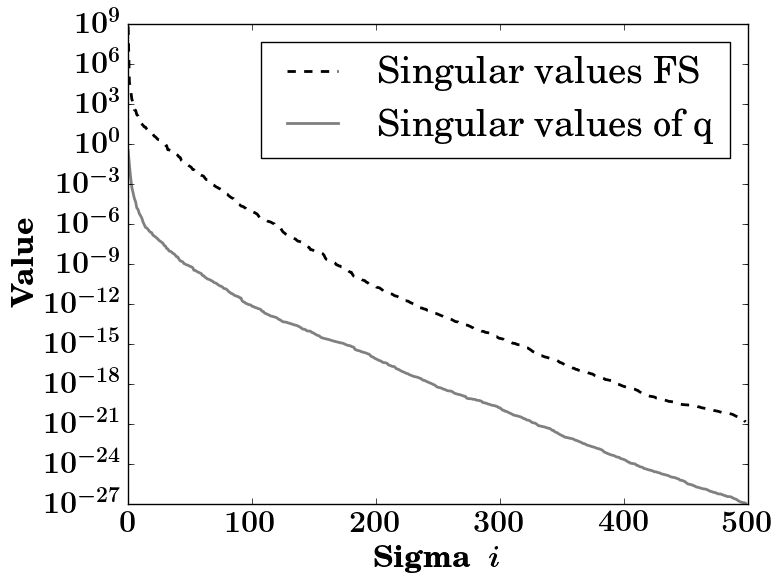
\includegraphics[width=0.6\textwidth]{singularvalues_last_year.png}
  \caption{Distribution of singular values from a SVD of $2880\_1_{3000}$, a matrix of snapshots of a full trajectory of the model year 3000.}
  \label{fig:singularvalues_last_year}
\end{figure}
The relative error of a run with a ROM, created out of the corresponding left singular vectors, over 3000 model years is visible in Figure \ref{fig:error_norm_last_year}.
The ROM $2880\_1_{3000}P150D150$ was initialized with an uniformly distributed concentration of $2.17 \frac{mmol}{m^3}$. The black line shows the relative error to the corresponding model year of the FOM.
The gray dashed line shows the relative error to state of the FOM in the model year 3000. Both are similar, very high and increasing most of the 3000 model years. Thus, starting with a uniformly distribution
does not lead to a usable behavior of the ROM. This is because the POD base projects the initial concentration vector on a low dimensional subspace, i.e. $V^Ty_0 = \hat{y}$, but the vector can not be well approximated in that
subspace.The approximation error $\parallel y_0 - VV^Ty_0 \parallel_2 = 234.3$ is very high. Thus, the initial projection leads to a large error of the ROM. 
\begin{figure}[ht]
\centering
  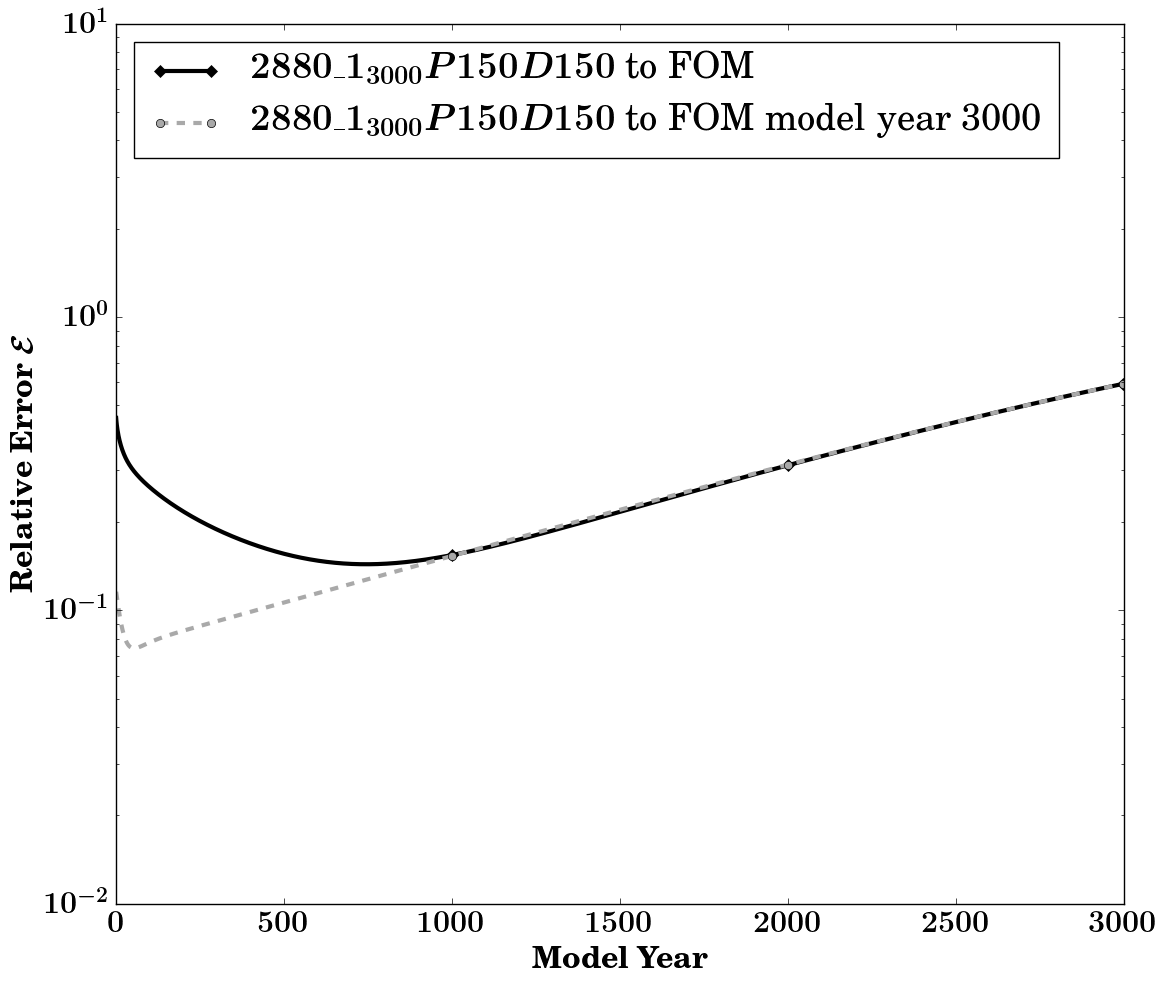
\includegraphics[width=0.8\textwidth]{error_norm_last_year.png}
  \caption[Relative error $\mathcal{E}$ of the reduced-order model $2880\_1_{3000}P150D150$ initialized with an uniformly distributed concentration to the FOM.]{Relative error $\mathcal{E}$ of the reduced-order model $2880\_1_{3000}P150D150$
	    initialized with an uniformly distributed concentration of $2.17 \frac{mmol}{m^3}$ to the FOM. The black line shows the relative error to the corresponding model year of the FOM.
	    The gray dashed line shows the relative error to state of the model year 3000 of the FOM.}
  \label{fig:error_norm_last_year}
\end{figure}
Initializing the ROM with a different concentration, which can be better approximated in the subspace spanned by the POD base, could lead to a better result. Therefore, 
the ROM was initialized with the solution of the FOM in model year 2000. The approximation error $\parallel y_{2000} - VV^Ty_{2000} \parallel_2 = 1.573$ is much smaller.
The relative error to the state of the FOM in model year 3000 is shown by the dashed gray line in Figure \ref{fig:error_norm_last_year_2000}. It is clearly visible that the ROM converges in the first 150 model years to the desired solution and diverges after that. Thus, it would be possible to use the solution of the ROM at that point, where the relative error has its minimum. Since the relative error can only be computed if the original solution is known, it would be more practical to select that point out of other information. 
\begin{figure}[ht]
\centering
  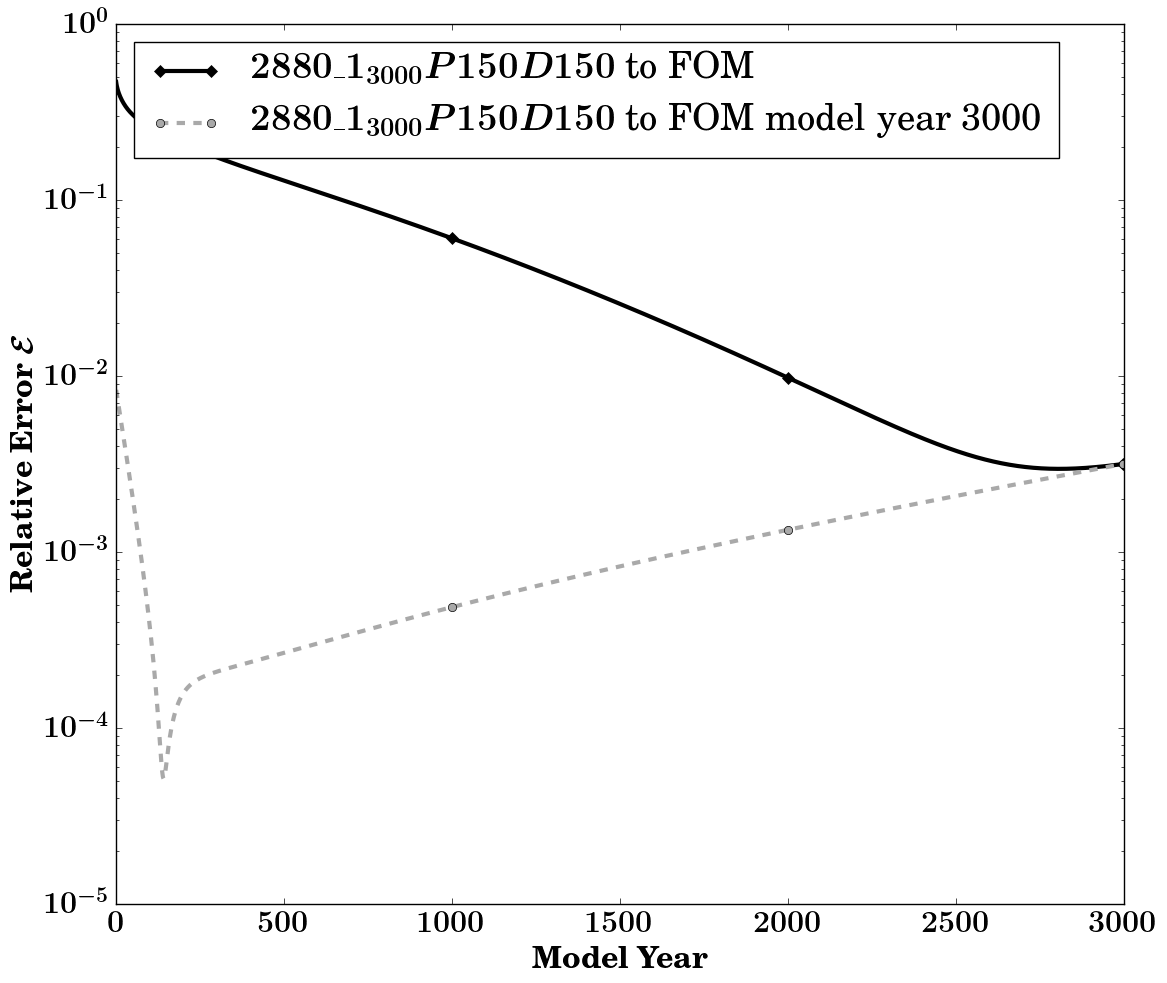
\includegraphics[width=0.8\textwidth]{error_norm_last_year_2000.png}
  \caption[Relative error $\mathcal{E}$ of the reduced-order model $2880\_1_{3000}P150D150$ initialized with the solution of model year 2000 of the FOM.]{Relative error $\mathcal{E}$ of the reduced-order model $2880\_1_{3000}P150D150$
	    initialized with the solution of model year 2000 of the FOM. The black line shows the relative error to the corresponding model year of the FOM.
	    The gray dashed line shows the relative error to state of the model year 3000 of the FOM.}
  \label{fig:error_norm_last_year_2000}
\end{figure}
The spin-up norm of this ROM shows an minimum at that point as well, visible in Figure \ref{fig:spinupnorm_last_year_2000}. It is not exactly the same point but it is quite close. The minimum of the relative error occurs in model year 141 and the minimum of the spin-up norm in model year 231. The information of the spin-up norm could be used to stop the ROM at the right model year to get an usable solution. Thus, a ROM created only with the trajectory of on model year can be used to generate a usable solution. It only has to be initialized with a concentration distribution that is closer to the one of the year the ROM was created with.
\begin{figure}[H]
\centering
  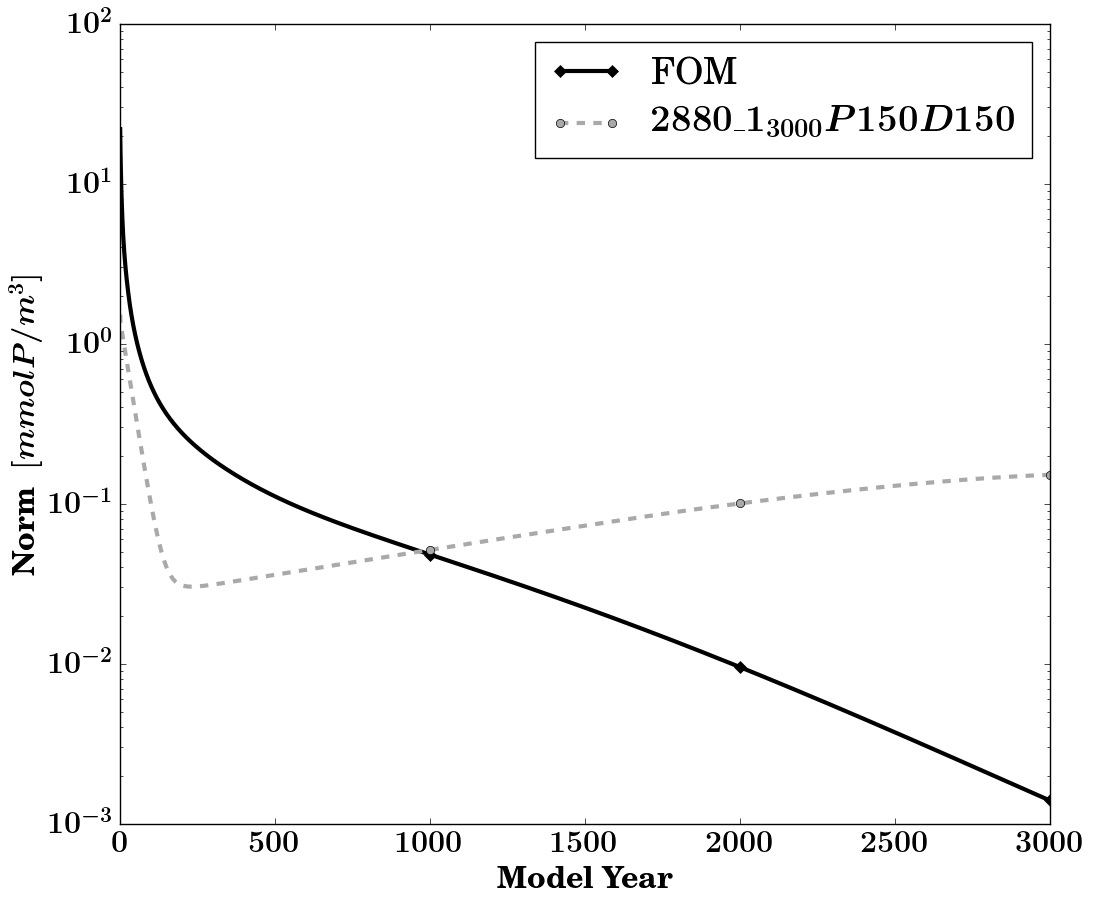
\includegraphics[width=0.8\textwidth]{spinupnorm_last_year_2000.png}
  \caption{Spin-up norm of the reduced-order model $2880\_1_{3000}P150D150$ in comparison with the spin-up norm of the full-order model.}
  \label{fig:spinupnorm_last_year_2000}
\end{figure}


\section{Implementation Issue} % Main appendix title

\label{AppendixA} % For referencing this appendix elsewhere, use \ref{AppendixA}
In the progress of this thesis, tests have shown that there is a small numerical difference in the matrix vector multiplication implemented in numpy and PETSc.
The same matrix vector operation has different results. This difference has been tracked down to the different order in which the addition in the matrix multiplication is performed. There, with some matrices vector combinations 
a difference of $4.44e^{-16}$ occurred, which is double the machine epsilon $\epsilon = 2.22e^{-16}$ for double precision floating point numbers. This happens because floating point additions are not necessarily associative.
In Figure \ref{fig:error_py_m3d} the absolute error between a model run in python and Metos3D is plotted. The example code and data can be found via
\begin{equation*}
 \text{\url{https://github.com/neeljp/matMult_error_python_petsc}.}
\end{equation*}
and can be used for further investigations at any time.

\begin{figure}[H]
\centering
  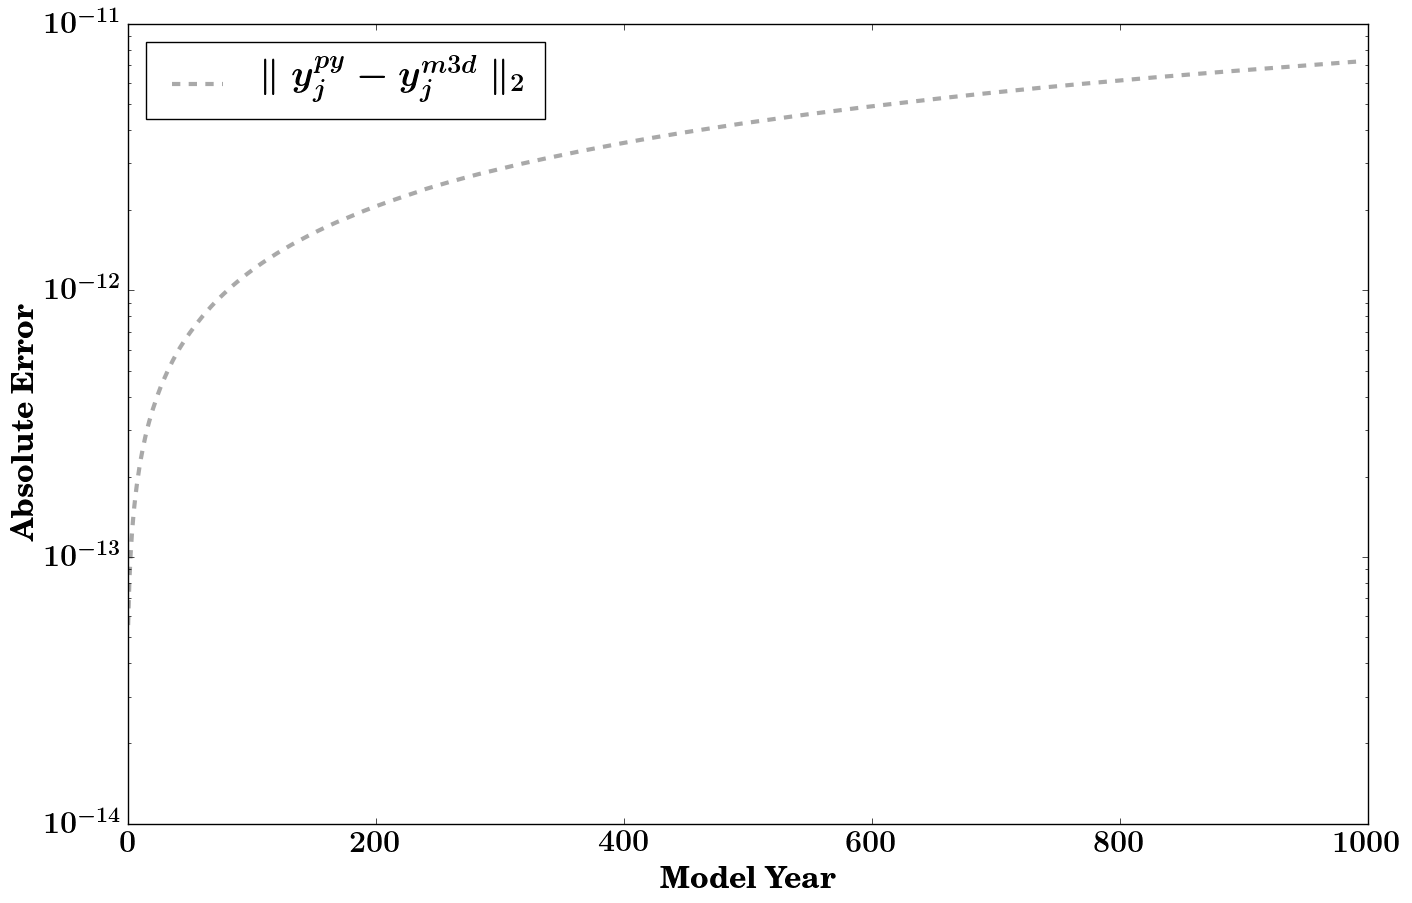
\includegraphics[width=0.9\textwidth]{error_norm_python_petsc.png}
  \caption[Absolute error of a model run with python and with PETSc]{Absolute error $\parallel y^{py}_j - y^{m3d}_j \parallel_2$ of a model run with python and with PETSc over 1000 model years.}
  \label{fig:error_py_m3d}
\end{figure}

\section{Distribution of the CPU time of the main operations of the ROMs} % Main appendix title
\label{Appendix:cpupie}
\begin{figure}[H]
\begin{subfigure}{.40\textwidth}
  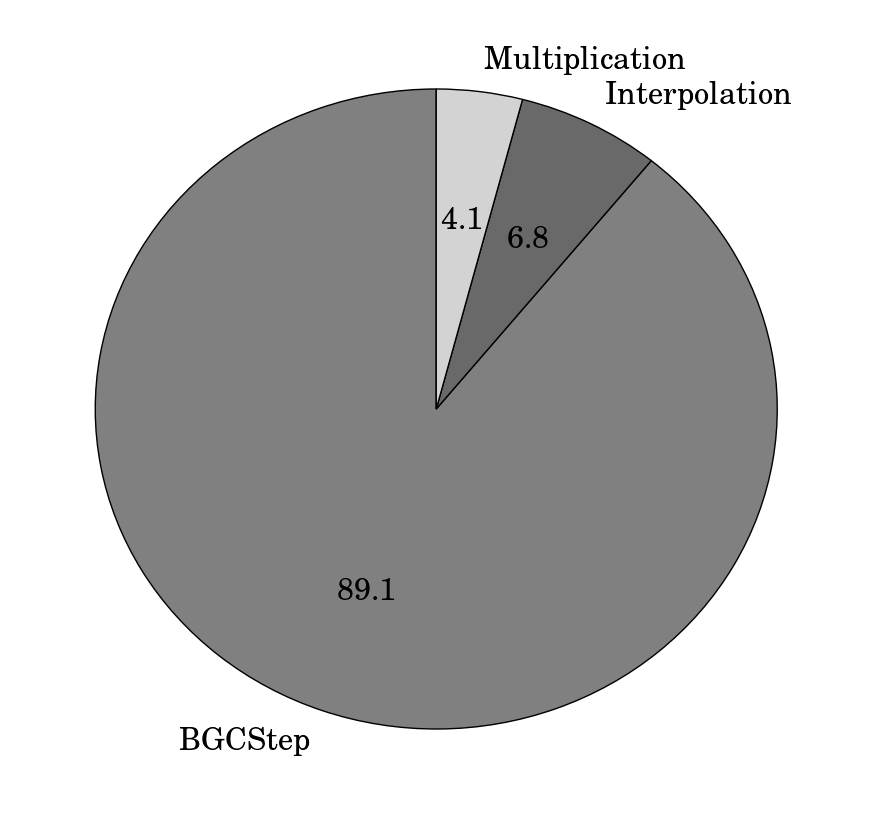
\includegraphics[width=1\textwidth]{timings_P100.png}
  \caption{Base POD100DEIM50}
  \label{fig:timings_sub1}
\end{subfigure}%
\begin{subfigure}{.40\textwidth}
  \centering
  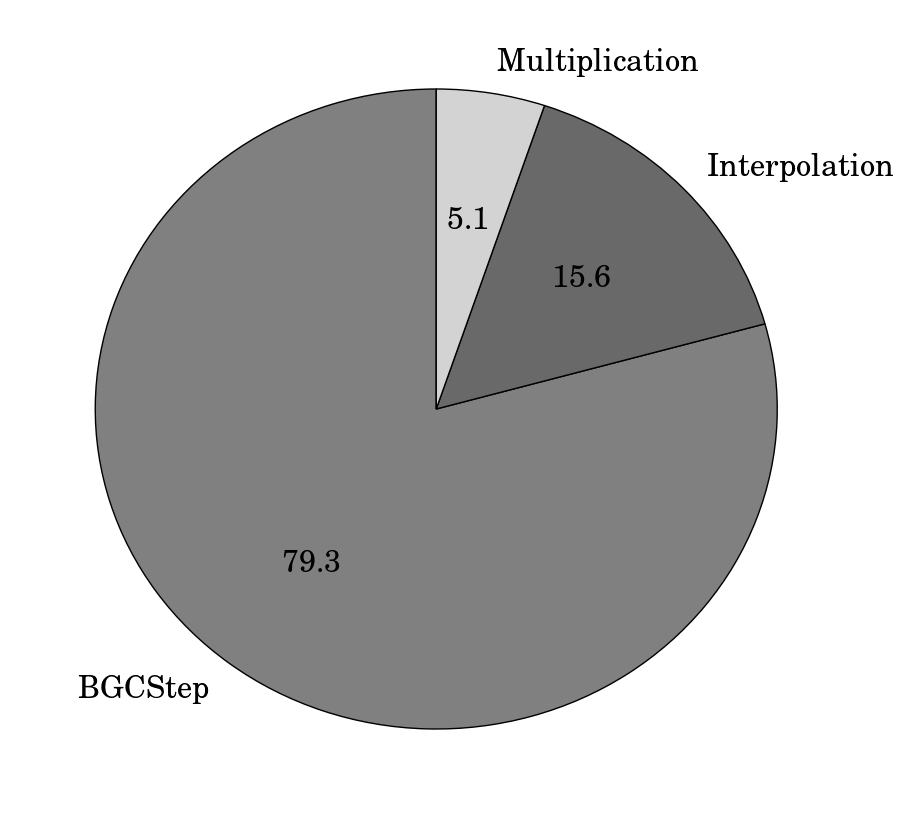
\includegraphics[width=1\textwidth]{timings_P300.png}
  \caption{Base POD300DEIM300}
  \label{fig:timings_sub2}
\end{subfigure}
\caption{Distribution of the computational time among main operations of the N-Model during the computation of a model year. The BGCStep part indicates the time that is needed to evaluate the nonlinear function.}
\label{fig:comparison_timings}
\end{figure}

\begin{figure}[H]
\begin{subfigure}{.48\textwidth}
  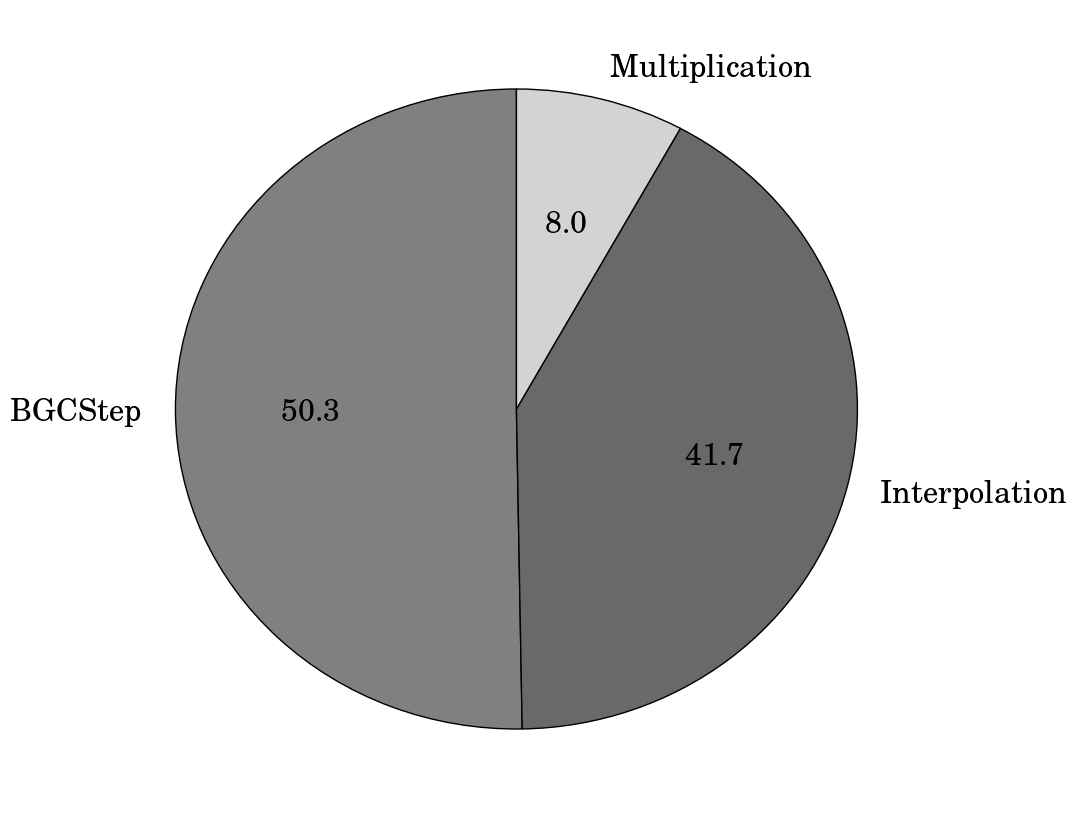
\includegraphics[width=1\textwidth]{timings_P100NDOP.png}
  \caption{Base POD100DEIM50}
  \label{fig:timings_N-DOPsub1}
\end{subfigure}%
\begin{subfigure}{.5\textwidth}
  \centering
  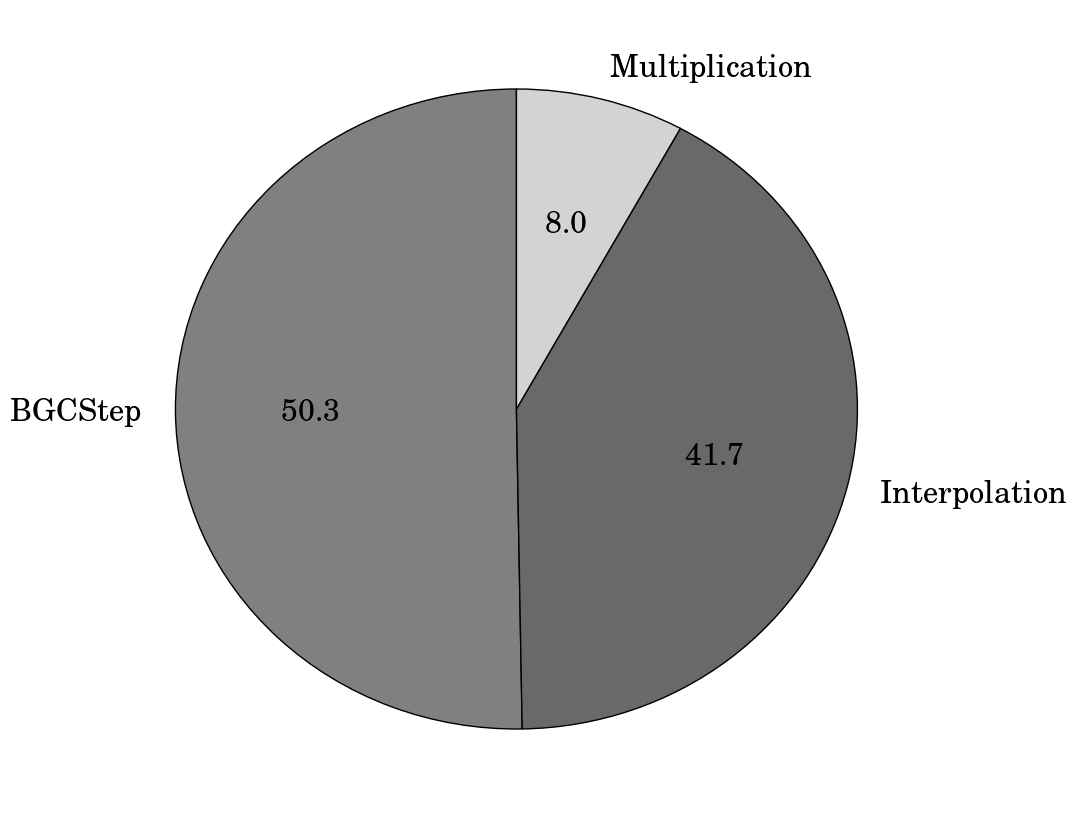
\includegraphics[width=1\textwidth]{timings_P100NDOP.png}
  \caption{Base POD300DEIM300}
  \label{fig:timings_N-DOPsub2}
\end{subfigure}
\caption{Distribution of the computational time among main operations of the N-DOP-Model during the computation of a model year.The BGCStep part indicates the time that is needed to evaluate the nonlinear function.}
\label{fig:comparison_timings_N-DOP}
\end{figure}

\section{Latin Hypercube samples}
\begin{table}[H]
\begin{center} 


$\begin{array}{|l|c|}
\hline
u_{LHC_0} & \{0.0470,140.86,1.305,17.078,0.891\}\\
\hline
u_{LHC_1} & \{0.0254,39.37,0.710,34.632,0.766\}\\
\hline
u_{LHC_2} & \{0.0405,175.83,0.392,19.928,1.251\}\\
\hline
u_{LHC_3} & \{0.0450,137.58,1.154,39.281,1.066\}\\
\hline
u_{LHC_4} & \{0.0289,113.77,0.594,26.857,1.488\}\\
\hline
u_{LHC_5} & \{0.0215,184.91,0.294,45.932,1.321\}\\
\hline
u_{LHC_6} & \{0.0332,58.38,1.473,24.204,1.363\}\\
\hline
u_{LHC_7} & \{0.0373,98.79,1.052,11.707,1.133\}\\
\hline
u_{LHC_8} & \{0.0121,63.83,0.787,46.016,0.828\}\\
\hline
u_{LHC_9} & \{0.0162,14.21,0.933,30.877,0.959\}\\
\hline
\end{array}$
\end{center}
\caption{10 Latin Hypercube samples used in Chapter \ref{Chapter5}.}
 \label{Chapter5:table_lhc_sample}
\end{table}

\section{Plots of parametrized models}

\begin{figure}[H]
\centering
  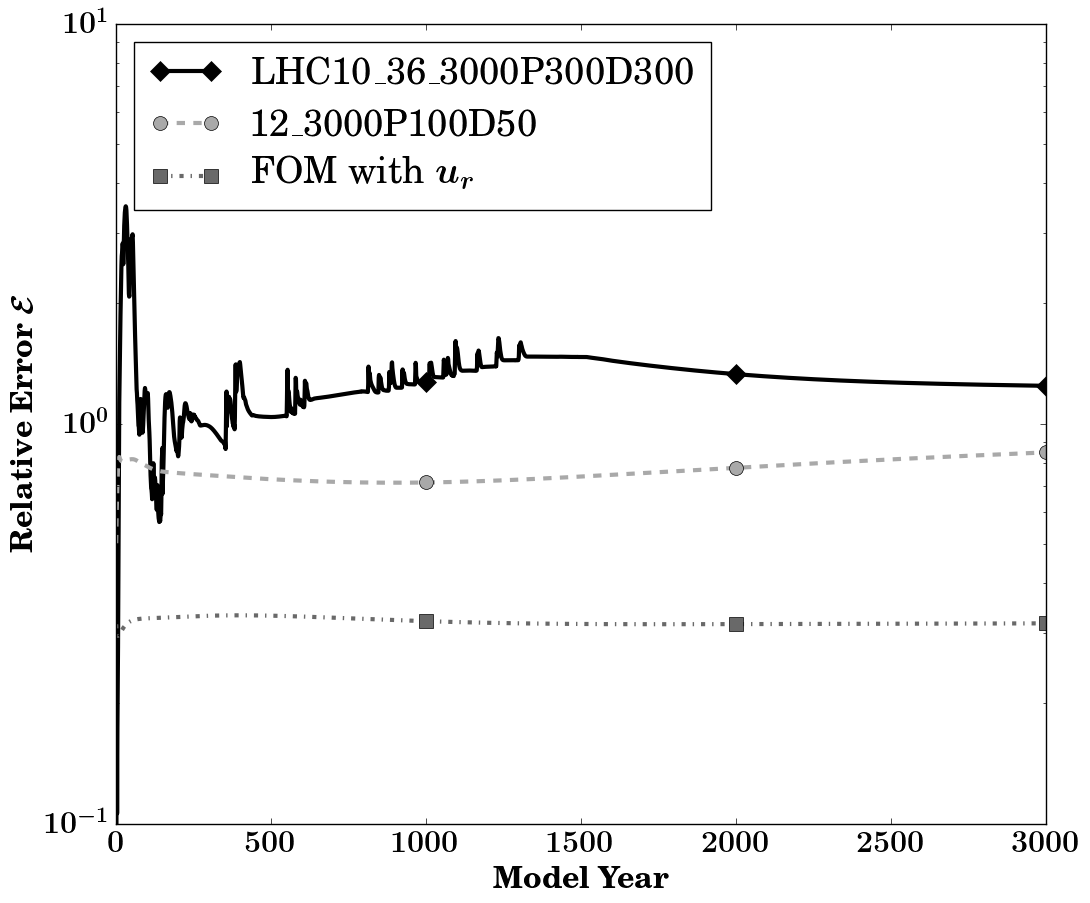
\includegraphics[width=0.9\textwidth]{error_norm_lhc_0.png}
  \captionsetup{width=1\textwidth}
  \caption[Relative error between different model runs and the FOM solution generated with $u_{LHC_0}$.]{Relative error between different model runs and the FOM solution generated with $u_{LHC_0}$. The black line is the relative error of the ROM generated with the
  ten Hypercube samples, run with $u_{LHC_0}$. The gray line with dots shows the relative error of the ROM out of Chapter 4 generated with the parameters set $u_r$, run with $u_{LHC_0}$.
  The dotted line with squares represents the relative error to the original solution of the FOM, run with parameter set $u_r$.}
  \label{fig:error_norm_lhc_0}
\end{figure}

\begin{figure}[H]
\centering
  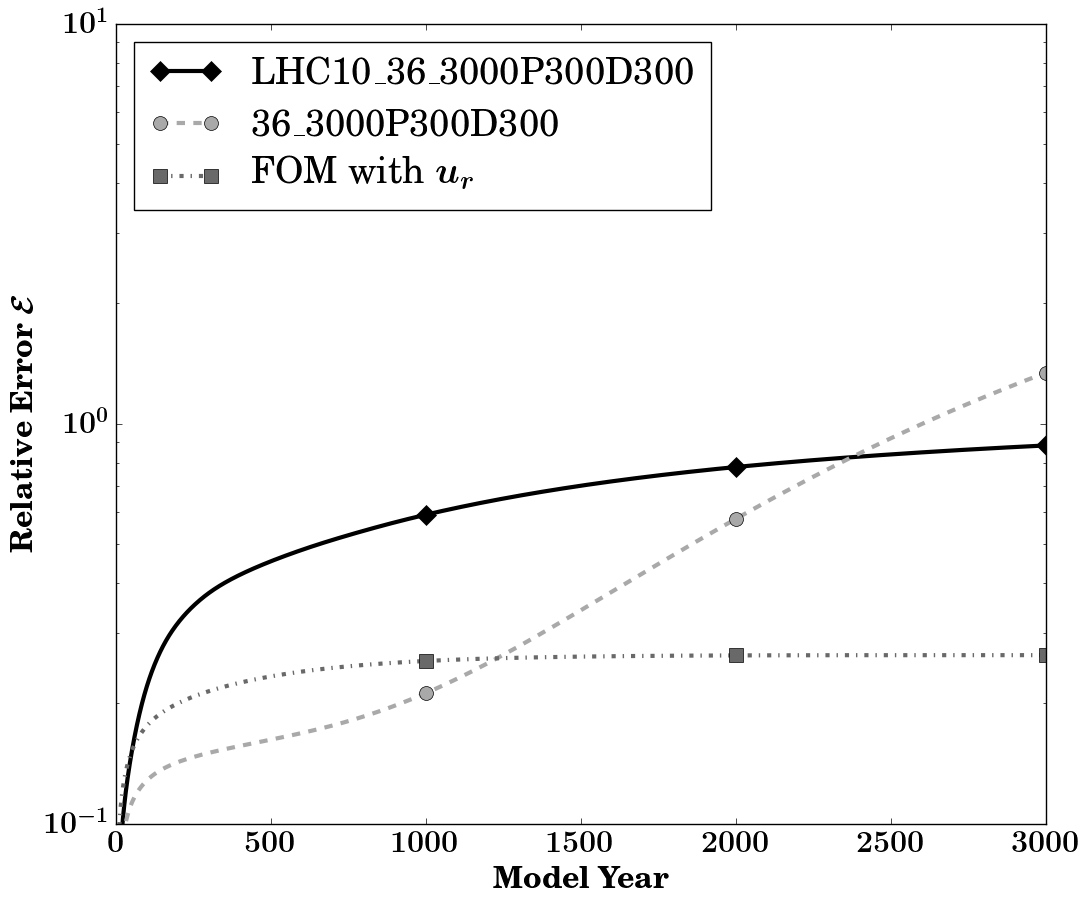
\includegraphics[width=0.9\textwidth]{error_norm_+50.png}
  \captionsetup{width=1\textwidth}
  \caption[Relative error between different model runs and the FOM solution generated with $u_r + 50\%$.]{Relative error between different model runs and the FOM solution generated with $u_r + 50\%$. The black line is the relative error of the ROM generated with the
  ten Hypercube samples, run with $u_r + 50\%$. The gray line with dots shows the relative error of the ROM $36\_3000P300D300$ out of Chapter 4 generated with the parameters set $u_r$, run with  $u_r + 50\%$.
  The dotted line with squares represents the relative error to the original solution of the FOM, run with parameter set $u_r$.}
  \label{fig:error_norm_+50}
\end{figure}


%\include{Appendices/AppendixB}
%\include{Appendices/AppendixC}

%----------------------------------------------------------------------------------------
%	BIBLIOGRAPHY
%----------------------------------------------------------------------------------------

\printbibliography[heading=bibintoc]

%----------------------------------------------------------------------------------------

\end{document}  
